 % %%%%%%%%%%%%%%%%%%%%%%%%%%%%%%%%%%%%%%%%%%%%%%%%%%%%%%%
% Please note that whilst this template provides a
% preview of the typeset manuscript for submission, it
% will not necessarily be the final publication layout.
%
%% Document class options: (**...** are defaults)
%  - bibtex: Uses bibtex+natbib, chicago.bst
%  - biblatex: Uses biblatex-chicago
%      You MUST select one of the above two options, depending
%      on whether you prefer bibtex or biblatex. This template
%      contains code that uses bibtex.
%  - twocolumn: Switch to two column for main text
%  - singlespace/onehalfspace/**doublespace**:
%         changes line spacing for main text
%  - **blind**/nonblind: Anonymises authors
%         and affiliations, or not
%  - autowc: Automatically inserts a word count
%         after the abstract, using texcount.
%         The abstract is ignored.
%%% autowc may cause longer compilation time. You can
%%% disable it first while actively editing, and only
%%% enable it when you're ready to take stock and check
%%% on your work.
\documentclass[bibtex,autowc,nonblind]{apsr_submission}
% \totalwordcount{500}

\title{Resurrecting \textit{Siege}: Collective Memory, Network Contagion, and Ideology Formation in the Iron March Neo-Fascist Forum}
\newcommand{\specialcell}[2][c]{%
  \begin{tabular}[#1]{@{}c@{}}#2\end{tabular}}
% The custom \author command takes THREE arguments:
% #1 = Author name
% #2 = Affiliation name
% #3 = Brief author profile, or anything that you'd usually put in a \thanks. Leave blank {} if there's nothing to be said.
\author{Alex Bradley Newhouse}
       {University of Colorado Boulder}
       {alex.newhouse@colorado.edu}

%% Any other acknowledgements or author notes

%% These are used for the headers
\runningtitle{}
\runningauthor{Alex B. Newhouse}

%% Useful packages
\usepackage{amsmath}
\usepackage{graphicx}
\graphicspath{{./}{../figures/}}
\usepackage{rotating}
\usepackage{svg}
\usepackage{caption}
\usepackage{booktabs}
%% If you are using a custom figure or table environment from a package and it's not getting framed, add \makeframedenv{MyFigure} in the preamble, where the custom figure environment is \begin{MyFigure}...\end{MyFigure}.

%% Handy for setting wide tables/figures in landscape
\usepackage{pdflscape}

%% Just to add some dummy text
\usepackage{lipsum}
\usepackage{ntheorem}
\newtheorem{hyp}{Hypothesis}
\newtheorem{subhyp}{Hypothesis}
   \renewcommand\thesubhyp{\thehyp\alph{subhyp}}
\newtheorem{prop}{Proposition}

\begin{document}
%%% DO NOT REMOVE THESE LINES. For automatic word count.
%TC:ignore
\begin{frontmatter}
\begin{abstract}
Decentralized online communities have become a common staging ground for offline political violence, yet the mechanisms linking forum activity to real-world mobilization remain underspecified. I develop a framework of \textit{collective memory-work}---the reputation-reinforced canonization, spatially concentrated exegesis, and peer-transmitted contagion of a textual artifact---to explain how decentralized online communities produce durable shared identity despite lacking formal hierarchy, fixed membership, or command structure. I test the framework using the 2015 republication of James Mason's neo-Nazi tract \textit{Siege} by administrator Zeiger on the Iron March forum (2011--2017), which became the constitutive text of a generation of militant accelerationist groups. Using the leaked database (195,128 forum posts, 21,715 private messages, and 272,129 reputation events), I estimate the republication's effects through interrupted time-series regression with heteroskedasticity- and autocorrelation-consistent errors, two-way fixed-effects panel models with node-label permutation inference, and Cox proportional-hazards survival analysis. The republication produced a persistent slope-driven structural break in forum rhetoric ($\beta_3=0.00015$, $p=0.001$, $R^2=0.46$). Forum co-participation exposure predicts user-level adoption ($\beta=1.13$, $p<0.001$), high-degree users adopt faster (hazard ratio $=2.92$), Siege-aligned posts receive 54 percent more reputation than comparable non-Siege posts, and rhetoric concentrates in interpretive and archival subforums (HHI $0.050 \to 0.116$). The three memory-work signatures appear jointly, while weekly Granger tests between Zeiger and the community fail to reject the null in either direction, inconsistent with a simple broadcasting model of ideological entrepreneurship.
\end{abstract}
\end{frontmatter}
%%% DO NOT REMOVE THIS LINE. For automatic word count.
%TC:endignore

\section{Introduction}

In 2015, the community on the Iron March web forum launched a neo-fascist zine called \textit{Noose}. Featuring writing from forum members, the zine promoted revolutionary fascism through historical retrospectives, philosophical treatises, and practical guides on cooking, orienteering, and prepping \citep{sunshine2024neo, upchurch}. Two years later, a small set of forum leaders resurrected a previously obscure 1980s publication called \textit{Siege}, written by an almost-forgotten neo-Nazi ideologue named James Mason. Repackaged with new art, commentary, and a preface from Mason himself, the Iron March edition of \textit{Siege} acquired an entire visual and rhetorical culture around it and became required reading for new recruits to Iron March-inspired offline groups.

These two initiatives were just two of many efforts by the Iron March network to construct a collective memory for the global neo-fascist movement. Events in the far past like the rise of Nazism, Mussolini's Fascist march, and the Italian Years of Lead were cast as pivotal moments in an ongoing revolutionary fascist project. The development of contemporary neo-fascism, in turn, was given a set of heroes, a coherent philosophy, and a trajectory that culminated in decentralized revolutionary violence, the tactics and strategies embodied by Iron March and its offspring groups.

Iron March is one of an increasing number of cases of highly decentralized online communities having a foundational impact on the development of offline social movements, political activism, and political violence. Among far-right online spaces, it is one of the most influential: its members established resilient cross-national ties \citep{upchurch}, launched a still-surviving genealogy of militant groups active in the United States, Canada, the United Kingdom, Europe, and Russia \citep{newhouse2021threat}, and provided a digital gathering-place for extremists who went on to commit arson, vandalism, and homicides \citep{singer2020iron}. The aesthetics of Iron March's version of neo-fascism have long outlasted the website itself, serving as connective tissue for extreme-right mobilization \citep{argentino2022one, colin2024and}. However, many other online communities have influenced offline violence, including 4chan's Politically Incorrect image board, the so-called Terrorgram network on Telegram, and involuntary celibate networks \citep{furstenberg2024decentralized}.

This paper contributes to the study of online extremism by developing and testing a theory of decentralized mobilization that centers on the collaborative production of collective memory. I argue that forum communities like Iron March can achieve enough cohesion to generate offline political violence despite having no formal hierarchy, no fixed membership, and no official organizational structure by collectively constructing a shared memory of past fascist movements and their heirs. The mechanism that binds the community together, in this account, is not deliberate top-down ideological entrepreneurship but a decentralized process of canonization, reinforcement, and exegesis organized around memory artifacts.

I use the 2015 republication of Mason's \textit{Siege} by the Iron March administrator Zeiger as a tractable event and test two sets of empirical claims. First, using interrupted time-series regression with heteroskedasticity- and autocorrelation-consistent standard errors \citep{bernal2017interrupted, newey1987simple}, the publication produced a persistent structural break in Iron March discourse. Second, using panel regression with fixed effects, node-label permutation inference, and Cox proportional-hazards survival analysis \citep{cox1972regression, shalizi2011homophily}, the rhetoric diffused through network exposure rather than through Zeiger's ideological entrepreneurship: network centrality strongly predicts earlier adoption, forum co-participation predicts subsequent user scores, and Granger-causality tests between Zeiger and the community fail to reject the null.

The argument is not that Iron March mobilized offline activism simply because it published a book. It is that the forum's infrastructure, its constitutional rules, its reputation mechanisms, and its thread-level interaction patterns constituted a memory-work apparatus that progressively canonized a particular text, built interpretive consensus around it, and stabilized a neo-fascist identity durable enough to survive the forum's own destruction. The remainder of the paper develops this theory, situates it in literatures on collective memory, social contagion, and online extremism, describes the measurement and identification strategy, and reports results from a battery of 11 primary tests on the Iron March corpus.

The paper restricts its dependent variable to ideological crystallization rather than offline violence itself. Other scholarship has documented the link from Iron March to specific attacks and organizations \citep{upchurch, newhouse2021threat, sunshine2024neo, ware2019siege, belew2018bring}; my contribution is to identify the forum-level processes that produce a coherent, action-oriented shared memory in the first place. The mobilization-to-violence pathway is a boundary condition discussed in the limitations, not a tested outcome.

\section{Decentralized Mobilization and the Puzzle of Collective Action}

Historically, the global far-right ecosystem has been organized around discrete groups like the Ku Klux Klan, the British National Front, or the Italian MSI. This has fundamentally changed over the past three decades. Concurrent with the rise of the Internet, far-right movements have increasingly embraced decentralization \citep{furstenberg2024decentralized, newhouse2021threat}, stochastic processes of mobilization \citep{conway2019right, amman2021stochastic}, and ``leaderless resistance'' as proposed by Louis Beam \citep{beam1992leaderless, kaplan1997leaderless}. This transformation of the structure of far-right violence has made it difficult to attribute attacks to broader organizations or movements, contributing to the acceleration of so-called lone-actor attacks \citep{gill2014bombing, ravndal2016right}.

As a growing body of scholarship has noted, however, these attackers are almost invariably anything but ``lone.'' They are immersed in and conversant with amorphous, highly decentralized swarm activity on extreme right-wing forums and online spaces \citep{tornberg2024echo, upchurch, kasimov2023decentralized, scrivens2023}. The puzzle that this creates for political science is acute. If there is no organization, no formal membership, no command structure, and no reliable disciplining mechanism, how do such communities produce the coordinated, motivated, and often sustained offline action that we observe? Classic resource-mobilization and collective-action theories presume at least some form of institution or organization capable of overcoming coordination and free-rider problems \citep{olson1971logic, mccarthy1977resource, tilly2017mobilization}. Iron March and its successors present a puzzle precisely because they appear to succeed at mobilization despite lacking the structures those theories identify as necessary.

Part of the answer lies in institutional design. Elinor Ostrom's framework for institutional analysis and recent work applying it to digital platforms \citep{ostrom1990governing, ostrom2004quest, frey2019_part, schneider} shows that even informal communities can develop stable constitutional, collective, and operational rules that reduce coordination costs. Another part lies in collective learning: scholars have shown that extreme-right and Islamist networks function as ``communities of practice'' that accumulate tactical and ideological knowledge through distributed participation \citep{kenney2020community, lee2022, furstenberg2024decentralized}. Neither answer is sufficient on its own. Institutional design explains why a community might persist, and collective learning explains how expertise circulates within it, but neither explains why some forums produce durable, action-oriented shared identity while others, structurally similar, do not.

My argument is that the missing ingredient is the production of collective memory around a textual artifact. Collective memory does two things that bear on the mobilization puzzle. First, it furnishes a shared narrative of who the community's ancestors were, what they fought for, and why their project remains unfinished, which can give members a reason to act on behalf of the group \citep{polletta1998contending, zamponi2013collective}. Second, it stabilizes identity across membership churn: new users arrive, old users leave, but the memory artifact persists and can be reread, reinterpreted, and recirculated \citep{hoskins2018memory, lundstrom2022temporal}. A community with strong collective memory can therefore sustain coordination even without a persistent organizational core, because its cohesion lives in the artifact rather than in the roster.

The distinction from communities of practice is worth making explicit. Communities of practice emphasize the tacit transmission of \textit{skills} through distributed expertise; they explain how tactical knowledge accumulates across a network. Collective memory, in the sense I use here, emphasizes the \textit{textually mediated} elaboration of a canonical narrative; it explains how identity and action-orientation stabilize across membership churn. The two framings are complementary rather than rival. An extremist network can be both a community of practice that circulates tactical knowledge and a memory community that curates a shared canon, and Iron March is plausibly both. My claim is more specific: what makes Iron March distinctive relative to structurally similar forums is not its tactical expertise but its memory-work.

The memory-work framework should also be distinguished from \textit{collective action framing} \citep{benford2000framing, snow1986frame, gamson1992talking}, which is the most natural rival account for the patterns I document. Framing theory treats narrative as strategic: movement entrepreneurs produce diagnostic, prognostic, and motivational framings designed to align prospective constituents with the movement's interpretation of the present. Memory-work, as I develop it, is non-strategic and retrospective: it is the distributed collective construction of the \textit{past} as an identity-stabilizing inheritance, organized around a textual artifact that the community can cite, interpret, and recirculate. The two accounts can be run on the same case with different predictions. Framing theory predicts entrepreneur-led flow: diagnostic framings originate with organizers and propagate outward. Memory-work predicts decentralized, exposure-driven adoption anchored in exegetical spaces rather than in entrepreneur-to-audience broadcasting. Section 8 shows the exegetical pattern; the Granger-null on Zeiger (the most visible entrepreneur) speaks directly to the rival-framing account.

\section{Collective Memory as Mobilization Infrastructure}

The study of collective memory is generally credited to \citet{halbwachs1992collective}, who conceived of a communal act of constructing a shared perspective on the past. Distinct from a \textit{history}, which is designed to accept complexity and multiple viewpoints, collective memory is the assertion of a shared viewpoint built around an opinionated infrastructure \citep{assmann1995collective, olick1999collective}. In a review of collective memory studies, \citet{wertsch2018collective} describes the development of ``schematic narrative templates'' that allow for the entrenchment of collective memory in a society, culture, or group. These templates can produce outcomes strong enough to induce ``memory inertia,'' in which certain collective memories become difficult to destabilize even when confronted with evidence challenging their core premises \citep{schuman2005elite}.

Collective memory processes play an important role in the development of social movements, allowing for the creation of group identity and the articulation of movement goals \citep{zamponi2013collective, kuo2024political}. Collective memory has been identified as a \textit{necessary} element for continuous mobilization: as \citet{lundstrom2022temporal} argue, collective memory ``mediation'' through different types of media produces differing outcomes, such as the production and re-production of memory frameworks over time. Because of its importance, fringe movements have actively weaponized new technologies to manipulate collective memory of the past and push for the entrenchment of beneficial perspectives of events such as the American Civil War or the Yugoslav wars \citep{wasilewski2023radical, ristic2024far}. As \citet{zamponi2013collective} puts it, ``Movements can challenge the hegemonic representation of their antecedents, as reported by the media, or distance themselves from them. A movement can adopt old symbols, traditionally far from its identity, and charge them with new meanings.''

Scholars in the human-computer interaction and broader information science traditions have applied the concept of collective memory to online communities by leveraging the availability of long-term digital trace data. Wikipedia has been identified as a hotspot of collective memory activity, because its structure is designed to produce collaboration in the construction of perspectives on events \citep{pentzold2009fixing, ferron2011collective, keegan2013hot}. Wikipedia visitors exhibit patterns of behavior indicative of collective memory formation via the consumption of articles in the neighborhood of those about current events \citep{garcia2017memory}, and editors diverge along language lines in their treatment of politically charged episodes such as the Arab Spring \citep{jones2024crosslanguageevolutiondivergentcollective}. Social media platforms have similarly been shown to shape new forms of historical consciousness among their users \citep{birkner2020collective, yasseri2022collective}. Despite the richness of this work, scant attention has been paid to the application of collective memory theory to online extremist movements specifically.

\subsection{Three Mechanisms}

By \textit{memory artifact} I mean a materially instantiated textual or visual object that a community can collectively cite, interpret, and recirculate as a durable anchor for shared memory. The usage follows Wertsch's treatment of textual mediational means \citep{wertsch2018collective} and Assmann's distinction between communicative memory (ephemeral, interactional) and cultural memory (durable, inscribed) \citep{assmann1995collective}. The 2015 Iron March edition of \textit{Siege} is the clearest example in this case. In Assmann's terms, the republication is the inscription moment that converts a communicative-memory substrate (diffuse, interactional forum chatter about Mason) into cultural memory (a fixed, citable, reproducible text). This distinction does theoretical work in what follows. It predicts that the structural break should appear as a slope, not a pure level, because inscription takes time to absorb and interpret.

I specify three mechanisms through which a decentralized community produces durable collective memory around such an artifact. The mechanisms are defined on different objects to keep them distinct.

\textbf{Canonization} operates on \textit{status}. It is the elevation of the artifact to a shared reference point that the community treats as authoritative. Canonization is observable in reward structures: if a reputation mechanism exists, canonized speech should attract disproportionate reputation. In a forum, the observable signature is excess reputation on canon-aligned posts.

\textbf{Exegesis} operates on \textit{interpretation}. It is the ongoing collective work of situating the artifact, explaining what it means, and contesting its application. A movement that merely names a text as important without interpreting it has a label, not a memory. In a forum, the observable signature of exegesis is spatial concentration of rhetoric in dedicated interpretive spaces (books, strategy, archives) where users curate and argue about meaning, rather than diffusion across casual channels.

\textbf{Contagion} operates on \textit{individuals}. It is the peer-to-peer transmission process by which specific users acquire the canonized artifact and its exegetic frame, rather than discovering them independently. Because the community has no formal training or membership, transmission must operate through exposure to alters who have already adopted. In a forum, the observable signature is that individual adoption is predicted by the Siege scores of a user's network neighbors, and that users with more neighbors adopt faster.

Together, these mechanisms constitute what I call \textit{collective memory-work}: the reputation-reinforced, spatially concentrated, peer-transmitted production of a shared interpretive frame organized around a memory artifact. Exegesis is the binding mechanism within this bundle. Canonization without exegesis produces a dead text; contagion without exegesis produces a jargon; only the combination of the three produces the action-oriented shared frame that can stabilize mobilization.

Because contagion and exegesis are both observed on the same forum co-participation graph (see Section 7), the network-exposure effect and the spatial-concentration effect are partially entangled empirically. A user who is pulled into an interpretive subforum is simultaneously exposed to Siege-aligned alters and to the venue of exegesis. The tests in Section 8 should therefore be read as evidence for the joint operation of the three mechanisms rather than as cleanly separable effects. I return to this in the Limitations.

An institutional substrate is a necessary precondition. For collective memory-work to happen in a decentralized community, the community needs legible rules and persistent venues in which repeated interpretive interaction can occur. This is where the Ostromian institutional-design literature connects to the memory-studies literature. Section 5 argues that Iron March's Charter and subforum structure provided exactly that substrate.

A corollary of the artifact-centered view worth flagging for future work is that collective memory should be portable. Because cohesion lives in the artifact rather than the platform, destroying the platform should redistribute rather than eliminate the memory, with the redistribution trajectory depending on where the human network migrates. Testing this prediction requires data from receiving platforms after the November 2017 Iron March shutdown and is beyond the scope of this paper; I return to it in the Conclusion as a natural extension.

The central empirical question of this paper is whether collective memory-work in the sense above, rather than top-down ideological entrepreneurship, characterizes the 2015--2017 trajectory of Iron March.

\section{The Iron March Case}

Iron March was founded in 2011 by a Russian-Uzbek named Alexander Mukhitdinov (usually referred to by his online pseudonym ``Alexander Slavros''), who had ties to the Russian military \citep{upchurch, newhouse2021threat}. Slavros launched the website as a replacement for the short-lived International Third Positionist Forum, his first foray into administering online neo-fascist networking.

Iron March was designed intentionally to be a ``digital campfire,'' a place where far-right extremists of many ideological persuasions could meet, collaborate, and discuss offline activities \citep{tornberg2024echo}. It was built in the tradition of other white supremacist and fascist campfire communities like Stormfront, but it aimed to be much more strategically coherent and ideologically disciplined \citep{caren2012social, de2008stormfront}. By the time it was taken down in late 2017, Iron March had helped coalesce a transnational, revolutionary neo-fascist movement that gave rise to a generation of street activists, training camps, and terrorist groups \citep{upchurch}. It produced its own textual and visual languages, unifying its movement under a common name and influencing successors well into the 2020s \citep{colin2024and, argentino2022one}.

\subsection{Case Selection}

Iron March functions as a \textit{pathway case} for collective memory-work as a mechanism of ideological crystallization within decentralized online communities (in the sense of Gerring 2007; Eckstein 1975), selected because its combination of features makes the hypothesized mechanism both most detectable and most falsifiable. Three features recommend it. First, the forum has an explicit institutional substrate (a formal Charter, a curated subforum structure, a reputation mechanism, and a durable moderator corps), which is the precondition the theory identifies for exegesis to occur. Many forums do not meet this condition; Iron March does. Second, there is a discrete, datable canonization event (Zeiger's June 2015 publication) that provides a clean pre-post window for interrupted time-series and panel analyses. Third, the leaked database provides essentially complete observability of the substrate, including private messages and reputation events that most platforms do not expose. Given these enabling features, confirmatory results support the theory within its stated scope conditions but provide limited leverage on whether the mechanism extends to communities lacking those features. Failure to observe the predicted signatures on Iron March, conversely, would be substantial evidence against the theory precisely because the case satisfies the pre-conditions it specifies.

The scope conditions follow directly. The theory generalizes most cleanly to communities with an institutional substrate, a discernible canonization moment, and a memory artifact. It generalizes less cleanly to purely ephemeral forums without curated rules or roles, to loosely federated messaging networks without a shared canonical text, or to platforms where reputation signals do not exist. Extending the framework comparatively is a natural next step and is discussed in the conclusion.

\subsection{Data}

The forum went offline on November 21, 2017 in a voluntary shutdown initiated by Slavros; a full snapshot of the site's database was subsequently posted online by an antifascist activist in November 2019 \citep{singer2020iron}. This database includes near-comprehensive information on the website's members, their direct messages, the forum threads and posts, and logs and metadata on the website's structure. It reveals that, despite primarily writing in English, Iron March users came from dozens of countries \citep{upchurch, singer2020iron, ross2019transnational}. All digital trace evidence presented in this paper comes from either this leaked database or from manual review of website snapshots stored by the Internet Archive's Wayback Machine.

The analysis uses six core tables from the leaked database: 195,128 forum posts, 7,182 forum threads organized into 144 subforums, 21,715 private direct messages, 1,207 members in the core members table (reconciled against an additional 763 in an earlier ``original'' members table), and 272,129 reputation events (likes and analogous reactions).

\subsubsection*{Data and ethics}

The Iron March corpus was obtained from a publicly available antifascist-activist leak that has circulated in open-web repositories since 2019 and has been used in multiple peer-reviewed studies \citep{upchurch, singer2020iron, ross2019transnational, sunshine2024neo}. This project received IRB review and was determined to involve data not obtained through interaction with human subjects; no identifying information beyond publicly adopted forum pseudonyms is reported, and no direct quotation is drawn from private messages involving minors. Replication code, the 54-term lexicon with weights, and the derived aggregate series will be released on a public Dataverse repository upon publication; the raw underlying corpus will not be redistributed, consistent with harm-minimization practice in extremism research.

\section{Structure and Affordances}

Before turning to the main statistical analysis, I briefly describe two features of Iron March's institutional design that are load-bearing for the argument: the Charter and the logo. Both are interpretable as memory-work in the Wertschian sense, because they situate the community at its inception as the heir to a particular 20th-century fascist genealogy.

\subsection{The Iron March Charter}

Iron March was launched in Fall 2011 with a small set of initial users and an overarching set of rules, called the Charter. This Charter was composed of language primarily ported over from Iron March's predecessor, ITPF. While various friends of Slavros contributed to it, its initial iterations were primarily the work of Slavros himself and his closest collaborator, Benjamin Raymond, a former British National Party youth figure who would co-found the British neo-fascist collective National Action in 2013 with Alex Davies \citep{macklin2018only, macklin2020failed}.

Applying the framework for institutional analysis developed by Elinor Ostrom and the Ostrom Workshop \citep{ostrom1990governing, ostrom2004quest, frey2019_part}, the Charter can be understood as an attempt at establishing a constitutional layer of rules and norms for the Iron March community. While all online communities have some set of rules to govern how users interact, much of the time these consist of low-level operational community guidelines and policies governing the allowable behaviors \citep{frey2019_part, schneider2022}. Iron March is distinct in its early adoption of a constitution that established the processes by which operational and collective rules could be made. It also established a vision for Iron March, defining who the community would be for and, perhaps more importantly for a neo-fascist network, who it would \textit{exclude}.

The Charter asserted these rules in part by initializing the Iron March community as an heir to a legacy of neo-fascist activism stretching back into the 20th century. Along with declaring operational guidelines, the Charter articulates the website's mission: ``Iron March is not a movement, but we expect users to share our purpose---to take an active interest in using the community, and when contributing to do so as fascists in ultimate pursuit of knowledge, ideas, contacts, etcetera,'' the earliest Charter from September 2011 states \citep{charter2011}. It also positions the website in opposition to white nationalist communities: ``This is not Stormfront. Our community is based on discussion and debate constructive towards fascist goals, it is not a hangout for White Nationalists and their unique subculture'' \citep{charter2011}. The Charter thus establishes Iron March as something more cohesive and directional than a ``hangout'' like Stormfront, but less unified than a social movement. Iron March aimed for creating a ``forum, an information center, and a community for like-minded people.'' Stormfront itself has an institutional substrate including graded moderator tiers and an extensive rules apparatus \citep{bowman2009, caren2012social}; the distinctive feature of Iron March's Charter is not merely procedural rule-making but its \textit{ideologically programmatic} exclusion of adjacent white-nationalist subcultures.

By the end of Iron March's existence, the website leadership had updated the Charter with a mission statement declaring the various strategic goals and tactics of Iron March. The statement establishes four main functions: forging the 21st century fascist, serving as a fascist alma mater, hosting fascist space, and constituting a fascist fraternity \citep{charter2017}.

\subsection{The ``Machina Hierarchia'' and the Aesthetic Brand}

\begin{figure}
    \centering
    \includesvg[width=.6\linewidth]{Logo_of_Ironmarch.org.svg}
    \caption{Flag of Iron March containing the ``Machina Hierarchia'' logo.}
    \label{fig:im-logo}
\end{figure}

The Charter positions the website in the legacy of past fascist and neo-fascist movements via the establishment of an aesthetic brand. Alongside roles and rules, the Charter specifically declares the ``Machina Hierarchia'' as the website's logo and seal, and only administrators and moderators are allowed to include the seal in their profiles. While this logo (Figure \ref{fig:im-logo}) is custom to Iron March, it is strongly inspired by historical fascist movements \citep{milleridriss2020hate}. The cogwheel at the middle of the logo was originally used by the Deutsche Arbeitsfront, the labor organization run by the Nazi Party following the Nazis' ascension to power in 1933 \citep{davis1994flags}. It has since been adopted by some neo-Nazi organizations, including the Hammerskins \citep{adl_hammerskins}. The hands superimposed on top of the cogwheel likely form a variant of the triskelion, an ancient symbol that was used by certain Nazi divisions and has been extensively employed by neo-Nazi movements \citep{dyck2016reichsrock}. The tree branches may have been taken from Nazi divisional flags. In addition to taking visual inspiration from the Nazi regime, the Charter also names the website's moderators an ``Order of Knights'' called the ``Black Corps,'' both references to nicknames for members of the Schutzstaffel (SS) division of the Nazi regime run by Heinrich Himmler.

These aesthetic decisions indicate an intentional cultivation of a shared ancestry for the Iron March project. Rather than use more ``mainstream'' fascist symbols such as the swastika or fasces, Iron March embraced the symbols of third-positionist and esoteric movements \citep{milleridriss2020hate}, which indicates a narrowness to Iron March's collective vision of both the past and the future that later showed up as Iron March users built offline groups \citep{upchurch}.

\section{Resurrecting \textit{Siege}}

Prior to 2015, neo-Nazi ideologue James Mason had largely been ignored by far-right movements globally since the height of his writing productivity in the 1980s. Mason's writings had not acquired much influence in shaping far-right mobilization and organization, and he was studied by social scientists more as a synthesizer of the far-right milieu than as a producer of ideology and movement politics himself \citep{johnson2023siege}. In one of the few pre-2015 studies of \textit{Siege}, \citet{goodrick2002black} argues that Mason should be understood as a reflection of the intersecting thought of Charles Manson, Ku Klux Klan leader Louis Beam, and other ideologues, rather than as an independently important figure. Mason was arrested in May 1994 on charges including sexual exploitation of a minor; the principal charges were subsequently reduced, and after a 1995 felony-menacing conviction in connection with the same case he served roughly three years in state prison, after which he largely withdrew from movement activity \citep{sunshine2024neo}. Mason's writings were occasionally discussed in extreme right-wing circles during the 2000s and early 2010s, but offline action, including violence, was more frequently attributed to texts like \textit{The Turner Diaries} by William Luther Pierce.

On June 3, 2015, Iron March user Zeiger (member ID 2170, later identified as the Canadian-based propagandist Gabriel Sohier-Chaput and already a core contributor to the \textit{Daily Stormer}) started a forum thread announcing that he had edited and revised \textit{Siege}. ``I've re-edited the whole book to a clean and fresh look, with standard page size, corrected spelling and punctuation errors and clean formatting,'' Zeiger, a member of the Black Corps, wrote as an introduction to this project. ``This is a huge step up from the garbage Solar General edition,\footnote{The Solar General edition was Mike Bean's digital archive version and was one of the only widely circulated versions of \textit{Siege} available at the time.} and the paper copies go for 150\$ these days.\ldots Every Ironmarch poster should read this book.'' Zeiger attached a PDF version and later updated the forum thread with an EPUB version, to enable compatibility with as many devices as possible. Sohier-Chaput was subsequently charged and, in 2022, convicted in Canada for wilful promotion of hatred in his \textit{Daily Stormer} writing; his pre-\textit{Siege} career as a multi-platform propagandist means that aggregate Iron March Granger-null results between Zeiger and the community (Section 8.2) should be read as evidence against a simple within-forum broadcasting model, not as a claim that Zeiger lacked influence beyond Iron March.

This newly updated edition of \textit{Siege} is branded with a title page declaring, ``An ironmarch.org publication,'' and its cover is a photograph from the Euromaidan protests in Ukraine in 2014. It includes a preface and introduction from the second edition published in 2003; the introduction, written by Nazi publisher Ryan Schuster, asserts that Mason's writings are ``so subversive and violent'' that other far-right extremists have been turned off of it \citep{siege2015}. This introduction aims to canonize Mason as a crucial figure in the legacy of neo-fascism, comparing him to Louis-Ferdinand C\'eline, whose antisemitic polemic \textit{Les Beaux Draps} was banned in Vichy France for its criticisms of the French military \citep{maftei2011ecriture}.

This effort to canonize Mason gained particular momentum in 2017, when Zeiger's third edition was updated with a new preface from Mason himself:

\begin{quote}
    Adolf Hitler, our greatest champion---as Rockwell would state---in two thousand years, declared in the course of his final radio broadcast to the German people, as well as to all the people of the White world, on January 30th, 1945, that with the victory of National Socialists over Bolshevism in Germany in 1933, the battle had been won and could not be reversed. Hard to believe then, hard to believe in 1967 or 1980. Maybe not so hard to believe today \citep{siege2017}.
\end{quote}

This new quote from Mason serves a dual purpose. First, Mason establishes a connection to a genealogy of revolutionary fascism stretching from himself to American Nazi Party leader George Lincoln Rockwell and originating with Adolf Hitler, white fascists' ``greatest champion in two thousand years.'' Second, Mason suggests that contemporary efforts in neo-fascist activism, specifically including Iron March, are the heirs of the Nazis who had won the battle for white power.

Qualitatively, Iron March's projects increasingly used the \textit{Siege} name and promoted their connections to Mason himself. In 2017, Iron March users launched an effort called Siege Culture which aimed to wrap a set of tactics and strategies in a unified aesthetic style. This involved the creation of two new affiliated websites (siegeculture.com and siegeculture.wordpress.com), the publication of numerous blog posts and essays, and the leveraging of memory artifacts for marketing and recruitment purposes.

Iron March users adopted the name and style of ``Universal Order,'' a short-lived group formed in 1982 by Mason with explicit inspiration from Charles Manson. The SiegeCulture.com banner reproduced in Figure \ref{fig:siegeculture} shows the Universal Order insignia (a swastika-crucifix) and the tagline ``Siege Culture,'' both of which circulated widely in the post-Iron March neo-fascist ecosystem. The name outlived Iron March itself and became used throughout the revolutionary neo-fascist ecosystem, including by militant groups with direct Iron March genealogy. Atomwaffen Division (transnational, founded in the U.S.), Feuerkrieg Division (transnational, founded in Estonia), Sonnenkrieg Division (U.K., a spinoff of National Action), and The Base (transnational, founded in the U.S.) all explicitly tied themselves to Universal Order and Siege Culture between 2018 and 2020, after Iron March had been closed \citep{newhouse2021threat, lee2022, ware2019siege}. Adjacent alt-right street formations such as Vanguard America and the Rise Above Movement overlapped personally and aesthetically with the Iron March social network but were not direct organizational spinoffs, a distinction I maintain throughout.

\begin{figure}
    \centering
    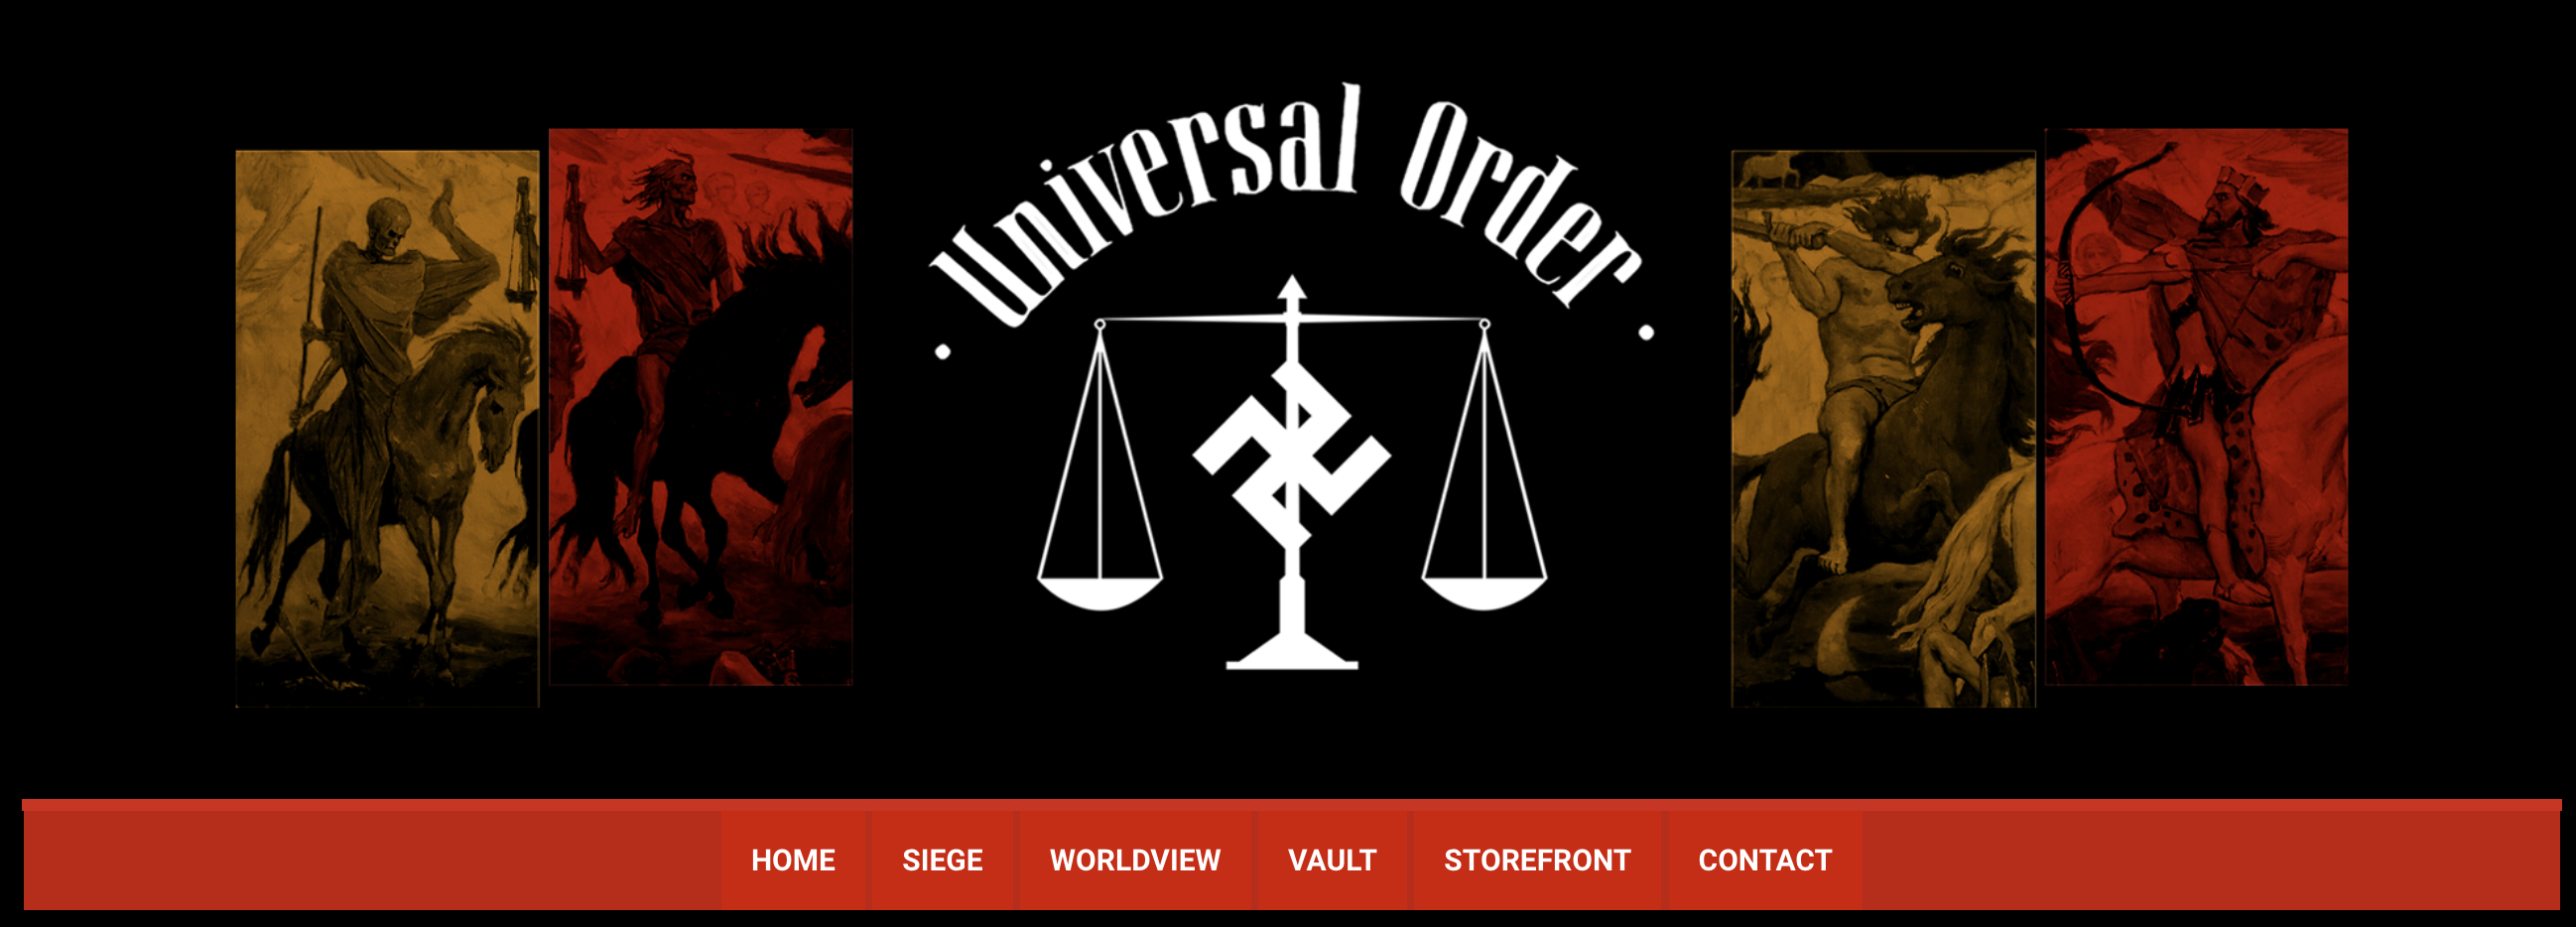
\includegraphics[width=0.5\linewidth]{image.png}
    \caption{Banner image from SiegeCulture.com in 2017.}
    \label{fig:siegeculture}
\end{figure}

Iron March users thus constructed a memory of James Mason and \textit{Siege} as the bridge between the knights of past fascist movements and Iron March's efforts to build a contemporary neo-fascist fraternity. Zeiger, Alexander Slavros, and the Siegist militant groups relied on this collective memory to mobilize. The narrative provided a common framing of both the past and the future that helped unify a geographically and ideologically disparate membership. The remainder of the paper tests whether this qualitative account is consistent with quantitative evidence from the forum corpus itself.

\subsection{Hypotheses}
\label{sec:hypotheses}

The three-mechanism framework of Section 3.1 (canonization, exegesis, contagion), combined with the Iron March case and the treatment event $T_0 = $ June 3, 2015, yields 11 observable implications that the empirical analysis tests. I organize them into four groups corresponding to the macro structural break, the meso contagion mechanism, canonization, and exegesis. Where the memory-work expectation diverges from the ideological-entrepreneurship or collective-action-framing rivals introduced in Section 3, I mark the divergence explicitly.

\paragraph{Macro: inscription as structural break.} If Zeiger's republication is the inscription moment that converts communicative memory (diffuse forum chatter about Mason) into cultural memory (a fixed, citable, reproducible text), it should mark a measurable discontinuity in forum-level Siege rhetoric. Because inscription takes time to be read, interpreted, and absorbed, the discontinuity should appear primarily as a slope change rather than a level jump.

\begin{hyp}[Structural break]
The weekly mean Siege rhetoric score on Iron March shows a persistent positive slope change after $T_0$, consistent with a gradual intensification driven by ongoing exegesis rather than a one-off level jump.
\end{hyp}

\paragraph{Meso: contagion and the entrepreneurship rival.} Memory-work predicts that Siege rhetoric diffuses through peer-to-peer exposure in the forum's public graph; the ideological-entrepreneurship rival predicts that the most visible individual (Zeiger) leads the community's weekly trajectory. Structural position in the graph should predict speed of adoption, newly joining users should arrive already saturated with the canon once it is established, and the forum (public) channel should lead the DM (private) channel if canonization is fundamentally a public performance.

\begin{hyp}[Network exposure]
User $i$'s monthly Siege score is positively predicted by the lagged mean Siege score of $i$'s forum co-participation neighbors, net of user and month fixed effects.
\end{hyp}

\begin{hyp}[Entrepreneur null]
Zeiger's weekly Siege score does not Granger-cause the rest of the community's weekly Siege score, contrary to a simple broadcasting model of ideological entrepreneurship.
\end{hyp}

\begin{hyp}[Cohort conversion]
Pre-$T_0$ joiners who post both before and after $T_0$ show positive within-user change in Siege score; post-$T_0$ joiners begin with higher Siege scores on their first posts than pre-$T_0$ joiners did on theirs.
\end{hyp}

\begin{hyp}[Forum-first pipeline]
Among users who use Siege-related language in both forum posts and direct messages, the forum-first pattern predominates, consistent with canonization as a public status-elevating act.
\end{hyp}

\begin{hyp}[Degree centrality]
Forum co-participation degree centrality predicts a shorter time-to-first-high-Siege-post in a Cox proportional-hazards model of adoption.
\end{hyp}

\paragraph{Micro I: canonization.} If the community does not merely tolerate but actively rewards canon-aligned speech, the reward signature should appear in the reputation-count data after adjusting for the mechanical confound of post length.

\begin{hyp}[Reputation reinforcement]
Siege-aligned posts receive more reputation than comparable non-Siege posts, net of log post length and month fixed effects.
\end{hyp}

\paragraph{Micro II: exegesis and convergence.} If the community performs collective interpretive work in dedicated spaces and converges semantically over time, four signatures should jointly appear: within-thread escalation of Siege content, thread-level exposure effects, a decline in between-user variance, and spatial concentration of Siege discourse in interpretive rather than social subforums.

\begin{hyp}[Within-thread escalation]
Within a given thread that contains any Siege content, post-level Siege rhetoric escalates with position in the thread.
\end{hyp}

\begin{hyp}[Thread-level exposure]
A user's Siege score in a given thread is positively predicted by the cumulative Siege content of posts that precede theirs within the same thread.
\end{hyp}

\begin{hyp}[Semantic convergence]
Monthly between-user variability in Siege scores (coefficient of variation) declines in the post-$T_0$ period, consistent with convergence on a shared interpretive frame.
\end{hyp}

\begin{hyp}[Spatial concentration]
Post-$T_0$ Siege rhetoric is more concentrated across subforums than pre-$T_0$, measured by the Herfindahl-Hirschman Index, and the subforums with the largest prevalence increase are interpretive and archival (e.g., books, archives, articles) rather than casual or social.
\end{hyp}

Section 7 describes the measurement and identification strategy for testing these hypotheses. Section 8 reports results. Table \ref{tab:scorecard} at the end of Section 8 summarizes the verdict on each.

\section{Measurement and Design}

The core empirical task is to measure, for each of 195,128 forum posts and 21,715 direct messages, how much the text expresses Siege-aligned ideology. That measurement then drives a family of time-series, panel, and survival analyses. Because the audience for this paper includes political scientists who may be less familiar with some of the specific techniques, I describe each method in enough detail to make the identification logic transparent, and I cite standard textbook treatments for readers who wish to consult the fuller econometric or computational-social-science literature.

\subsection{Measuring Siege Rhetoric}

The problem of quantifying a specific ideological orientation in short text is familiar in political science \citep{laver2003extracting, grimmer2013text, young2012affective, gentzkow2019text}. The simplest approach is a keyword dictionary: count mentions of words that are distinctively associated with the ideology. The weakness of pure dictionary scoring in extremist corpora is that the most diagnostic words (``siege,'' ``the system,'' ``collapse,'' ``total war'') are heavily overloaded with non-extremist meanings. A post about the Siege of Leningrad, a video game called \textit{Total War}, or the phrase ``the system isn't working'' can be wrongly scored as Siege-aligned.

I therefore combine two complementary measures \citep{rodriguez:2022a}.

\textit{Dictionary score.} I use a 54-term weighted lexicon organized into three tiers, supplemented with a small set of counter-indicators. Tier 1 contains unambiguous Siege markers with weights 1.0--3.0 (most at 2.5--3.0), such as \texttt{james mason}, \texttt{read siege}, \texttt{atomwaffen}, \texttt{universal order}, \texttt{joseph tommasi}, and \texttt{skull mask}. Tier 2 contains Siege-adjacent ideology and figures with weights 1.5--2.5, such as \texttt{accelerationism}, \texttt{leaderless resistance}, \texttt{day of the rope}, \texttt{charles manson}, and \texttt{william luther pierce}. Tier 3 contains context-dependent terms with weights 0.3--1.0 that are routed through an embedding-based context adjustment (see below). A small set of counter-indicators with negative weights reduces false positives (for example, the word ``manson'' appearing near ``Shirley'' or ``family'' usually references Shirley Manson of the band Garbage or the Manson family in an entertainment context).

\textit{Embedding score.} Each post is embedded using the \texttt{all-MiniLM-L6-v2} sentence-transformer model \citep{reimers2019sentence, devlin:2019}, which produces a 384-dimensional vector representation of the post's meaning. A reference centroid is computed as the mean embedding of a curated Siege corpus, which includes Mason's original writings, Siege Culture blog posts, and known Siege-aligned militant manifestos. Each post's alignment with the Siege centroid is measured as the cosine similarity between its embedding and the centroid \citep{manning2008introduction}. Cosine similarity ranges from $-1$ to $1$ and is scale-invariant; for short text domains, it is the standard proximity measure \citep{grimmer2013text}.

\textit{Embedding-boosted hybrid.} The dictionary and embedding scores address different weaknesses. The dictionary is precise on rare Tier 1 markers but brittle on Tier 3 overloaded terms; the embedding is robust to overloading but less sensitive to specific rare vocabulary. I combine them by letting the embedding similarity modulate the Tier 3 dictionary weights: a post containing ``the system'' in a neighborhood of high Siege embedding similarity receives a boost to its Tier 3 contribution, while the same phrase in an unrelated context is attenuated. The design follows a growing literature arguing that lexicon-plus-embedding measures outperform either alone on short and domain-specific text \citep{rodriguez:2022a}. Each post receives two scores: a continuous ``siege keyword score'' and a continuous ``siege similarity score,'' together with a binary ``siege post'' indicator based on a keyword threshold.

\subsection{The Treatment Event and Identification}

I treat Zeiger's forum post of June 3, 2015 publishing the Iron March edition of \textit{Siege} as the treatment event ($T_0$). The language of ``treatment'' here should be read in the interrupted-time-series sense of a shock that divides the series into pre- and post-periods \citep{bernal2017interrupted, wagner2002segmented}, not in the randomized-experiment sense of a research-assigned intervention. To avoid mechanical feedback, Zeiger's own posts are excluded from all time-series and network models. The forum continued operating until November 21, 2017, bounding the observation window at roughly 29 months of post-treatment data.

The identification logic rests on two conditions. The first is that the publication date is not endogenous to a simultaneous exogenous shock that would on its own produce the observed post-$T_0$ trajectory. The most visible candidate concurrent shock is the 2014 Ukraine conflict and the Azov Battalion's incorporation into the Ukrainian National Guard in November 2014, together with the Misanthropic Division recruitment pipeline that mobilized Iron March-adjacent fighters for the Donbas war \citep{colborne2022fires}. This Ukraine-war pipeline is proximal to, rather than cleanly separable from, the pre-$T_0$ drift that the PELT changepoint analysis identifies around June 2014 and March 2015 (Section 8.1). It is therefore a plausible \textit{parallel} driver of the 2014--2015 escalation in Iron March rhetoric rather than a cleanly bracketed shock, and I cannot fully rule it out; I return to this rival mechanism in the Limitations. The Charlottesville-era alt-right cycle, by contrast, peaked in August 2017 (more than two years after $T_0$) and is better read as a candidate \textit{consequence} of the Iron March-centered acceleration than as a cause. The second concern is endogeneity in the opposite direction: Zeiger's editorial timing may have been influenced by an internal Iron March shift already underway. Consistent with this, PELT identifies pre-$T_0$ inflections around June 2014 and March 2015, and the qualitative record shows increasing Siege-related activity across 2014--2015 (including the \textit{Noose} zine launch in spring 2015). I interpret these as evidence of a gradual, exegesis-driven build-up rather than a cold-start ignition at $T_0$, which is consistent with the theory but also means that the post-$T_0$ effect should be read as a \textit{decisive acceleration of an already-drifting series} rather than as the entry of a previously absent variable.

The second identification condition is the absence of anticipation. A pre-$T_0$ spike in Siege rhetoric that precedes the publication by weeks would suggest that community members knew the release was imminent and began conditioning their behavior on it. The forum corpus shows no such spike. Zeiger's project was not pre-announced, and the pre-$T_0$ drift identified above is a gradual trend rather than a step change preceding $T_0$. Under these two conditions, the segmented-regression estimates of the level change $\beta_2$ and the slope change $\beta_3$ can be interpreted as the effect of inscription and its subsequent exegesis, rather than as a spurious artifact of endogenous timing or anticipation.

\subsection{Analytic Strategy}

The hypothesis battery is organized around three levels of analysis: macro time-series, meso network contagion, and micro exegesis mechanisms. Table \ref{tab:scorecard} summarizes the 11 primary tests. The argument does not depend on any single test but on the pattern across them. The methods are described here; the results for each test appear in Section 8.

\subsubsection{Macro: Interrupted Time Series}

The central macro question is whether Zeiger's publication produced a structural break in Iron March discourse. The segmented-regression interrupted time-series model is a standard tool for this in epidemiology and policy evaluation \citep{wagner2002segmented, bernal2017interrupted}. On weekly means of the Siege rhetoric score, I estimate

\[
y_t = \beta_0 + \beta_1 t + \beta_2 D_t + \beta_3 (t - t_0) D_t + \varepsilon_t,
\]

where $y_t$ is the weekly mean Siege score, $t$ indexes weeks, $D_t$ is an indicator for weeks after $T_0$, and $(t - t_0) D_t$ is the number of weeks elapsed since $T_0$ (zero before). The coefficient $\beta_2$ captures an immediate level jump at $T_0$; $\beta_3$ captures a change in slope after $T_0$. A positive $\beta_3$ with a small or non-significant $\beta_2$ corresponds to gradual intensification after the treatment, which is what the collective memory-work theory predicts: a memory artifact takes time to absorb and interpret.

Weekly social-media counts typically exhibit autocorrelation, which violates the independence assumption of OLS standard errors and biases inference toward false positives. I use heteroskedasticity- and autocorrelation-consistent (HAC) standard errors following \citet{newey1987simple}, with a lag of 4 weeks (the standard rule-of-thumb for monthly-horizon autocorrelation in weekly data, roughly $4 (N/100)^{2/9} \approx 5$ for $N = 324$ \citep{newey1994automatic, hamilton1994time}). I supplement the parametric ITS with the PELT changepoint-detection algorithm of \citet{killick2012optimal}, which identifies optimal breakpoints in the series without requiring $T_0$ as an input, as a sanity check on the timing of the break.

To test whether Zeiger individually drove the community's subsequent rhetoric, I estimate bivariate Granger-causality tests between Zeiger's weekly Siege score and the community's (excluding Zeiger). Granger causality asks whether lags of one series improve the forecast of another, beyond that series' own lags \citep{granger1969investigating, hamilton1994time}. It does not establish causality in a structural sense, but it does constrain the space of plausible causal models: an absence of Granger flow from Zeiger to the community is consistent with decentralized adoption and inconsistent with a simple broadcasting model. I report $F$-statistics and $p$-values across lags 1--8.

\subsubsection{Meso: Network Contagion and Survival}

If Siege rhetoric diffuses through interaction rather than being independently discovered by each adopter, individual adoption should be predicted by exposure to already-adopting alters \citep{rogers2003diffusion, valente1996network, centola2010spread, christakis2007spread}. I construct three networks from the Iron March data: a forum co-participation network (edge between two users if they posted in the same thread), a direct-message network (edge if two users shared a private conversation), and a reputation network (edge if one user gave reputation to another's post). Edges are undirected and unweighted in the panel model; edge weights are used only for network description.

For each user $i$ and each month $t$, I compute a lagged exposure variable
\[
E_{i,t}^{(N)} = \frac{1}{|N(i)|} \sum_{j \in N(i)} s_{j, t-1},
\]
where $N(i)$ is $i$'s neighbor set in network $N$ and $s_{j, t-1}$ is $j$'s Siege score in month $t-1$. I then estimate a panel regression of $s_{i,t}$ on the three exposures with two-way fixed effects for users and months, implemented via within-transformation \citep{wooldridge2010econometric, angrist2009mostly}. User fixed effects absorb time-invariant user characteristics (persistent ideological predispositions); month fixed effects absorb platform-wide time shocks. A positive and significant forum-exposure coefficient means that controlling for persistent user traits and for time, users whose neighbors became more Siege-aligned last month are themselves more Siege-aligned this month.

The central identification threat is homophily: users with similar ideological tastes cluster in the same threads, so even without any influence, their scores co-move \citep{shalizi2011homophily, aral2009distinguishing}. Two-way fixed effects attenuate but do not eliminate this confound. As an additional robustness check, I perform a node-label permutation test \citep{gonzalez2014assessing} in which user identities are randomly shuffled 200 times across the observed network, breaking the link between each user's true ideological profile and their network position. The distribution of permuted exposure coefficients provides a non-parametric null; if the observed coefficient lies in the extreme tail of this distribution, the result cannot be attributed purely to observed network structure. This test addresses a specific kind of confounding (structural coincidence) but does not rule out latent-attribute homophily on unobservables.

I then estimate a Cox proportional-hazards model \citep{cox1972regression, therneau2000cox, allison2014event} of time to each user's first high-Siege post. The Cox model is the standard survival-analysis tool for event-history data with censoring; it estimates the instantaneous hazard rate of the event as a function of covariates, without requiring a parametric form for the baseline hazard. Covariates are standardized degree centrality, standardized betweenness centrality \citep{freeman1977set}, and standardized reputation. Hazard ratios (HRs) are exponentiated coefficients and are interpretable directly: a hazard ratio of 2 on degree centrality means that a one-standard-deviation increase in degree roughly doubles the instantaneous rate of adoption. Standard errors are partial-likelihood.

Finally, a cohort-adoption test compares user-level pre-vs-post Siege scores within the subset of users who joined before $T_0$ and posted both before and after, and compares the distribution of first-post Siege scores between pre-$T_0$ and post-$T_0$ joiners. These are simple $t$-tests and Mann-Whitney tests and are included because they speak to a different mechanism (conversion among continuing users versus recruitment of already-aligned new users) than the network contagion models do.

\subsubsection{Micro: Exegesis Mechanisms}

I test three observable implications of the collective memory-work argument.

\textit{Canonization.} If the community rewards Siege-aligned speech, Siege posts should receive more reputation than comparable non-Siege posts. Reputation-count data is over-dispersed (variance much greater than mean), which rules out Poisson regression. I therefore estimate a negative binomial regression \citep{hilbe2011negative} of reputation count on a Siege indicator, controlling for log post length and month fixed effects. The coefficient of interest exponentiates to an incidence rate ratio (IRR), interpretable as the multiplicative change in expected reputation associated with being Siege-aligned, holding length and month constant.

\textit{Spatial concentration.} If the community performs interpretive work in dedicated spaces rather than diffusing Siege rhetoric across all channels, Siege rhetoric should be more concentrated across subforums after $T_0$ than before. I measure concentration with the Herfindahl-Hirschman Index (HHI) \citep{hirschman1964concentration}, defined as the sum of squared subforum shares of all Siege posts, ranging from near 0 (perfectly diffuse) to 1 (all concentrated in one subforum). I report HHI pre- and post-$T_0$ and list the subforums with the largest pre-to-post increase in prevalence as a descriptive complement.

\textit{Semantic convergence.} If the community converges on a shared interpretive frame, the between-user variability in Siege scores should decline over time. I compute the monthly coefficient of variation (standard deviation divided by mean) of user-level Siege scores, and estimate an ITS on this series. A negative post-$T_0$ slope would be consistent with convergence. Because the coefficient-of-variation metric is itself sensitive to changes in the mean, and because heterogeneity decline is consistent with both exegesis (convergence on shared meaning) and contagion (common exposure driving common scores), I treat this test as joint evidence for exegesis plus contagion rather than for exegesis alone.

\subsection{Multiple Testing and Robustness}

The battery contains 11 primary hypothesis tests. Naive $p$-values on multiple correlated tests overstate significance \citep{benjamini1995controlling}. I report naive $p$-values in the main results and, in the scorecard, note which findings survive a Benjamini-Hochberg false discovery rate correction at $q = 0.05$. Because most supported findings are significant at $p < 0.001$, the FDR correction changes the verdict on only the borderline tests (H9 and H10).

\section{Results}

\subsection{Structural break in forum rhetoric (H1)}

Figure \ref{fig:its} shows the weekly mean Siege rhetoric score on Iron March between 2011 and 2017, with a vertical marker at the $T_0$ publication date. Segmented regression on the forum keyword score yields a slope change $\beta_3 = 0.00015$ ($p = 0.001$, $R^2 = 0.46$), corresponding to a persistent acceleration after June 2015. The level change $\beta_2$ is small and not significant for the keyword score ($-0.018$, $p = 0.40$) but is significant and negative for the similarity score ($\beta_2 = -0.026$, $p < 0.001$), which is consistent with a model in which the community does not flip overnight but gradually intensifies its Siege rhetoric over the following two years. Pooling the forum and DM channels into a combined score raises the $R^2$ to $0.51$ while preserving the slope acceleration ($\beta_3 \approx 0.00014$, $p < 0.001$). PELT changepoint detection identifies an inflection around September and October 2015, roughly four months after the publication.

\begin{figure}
    \centering
    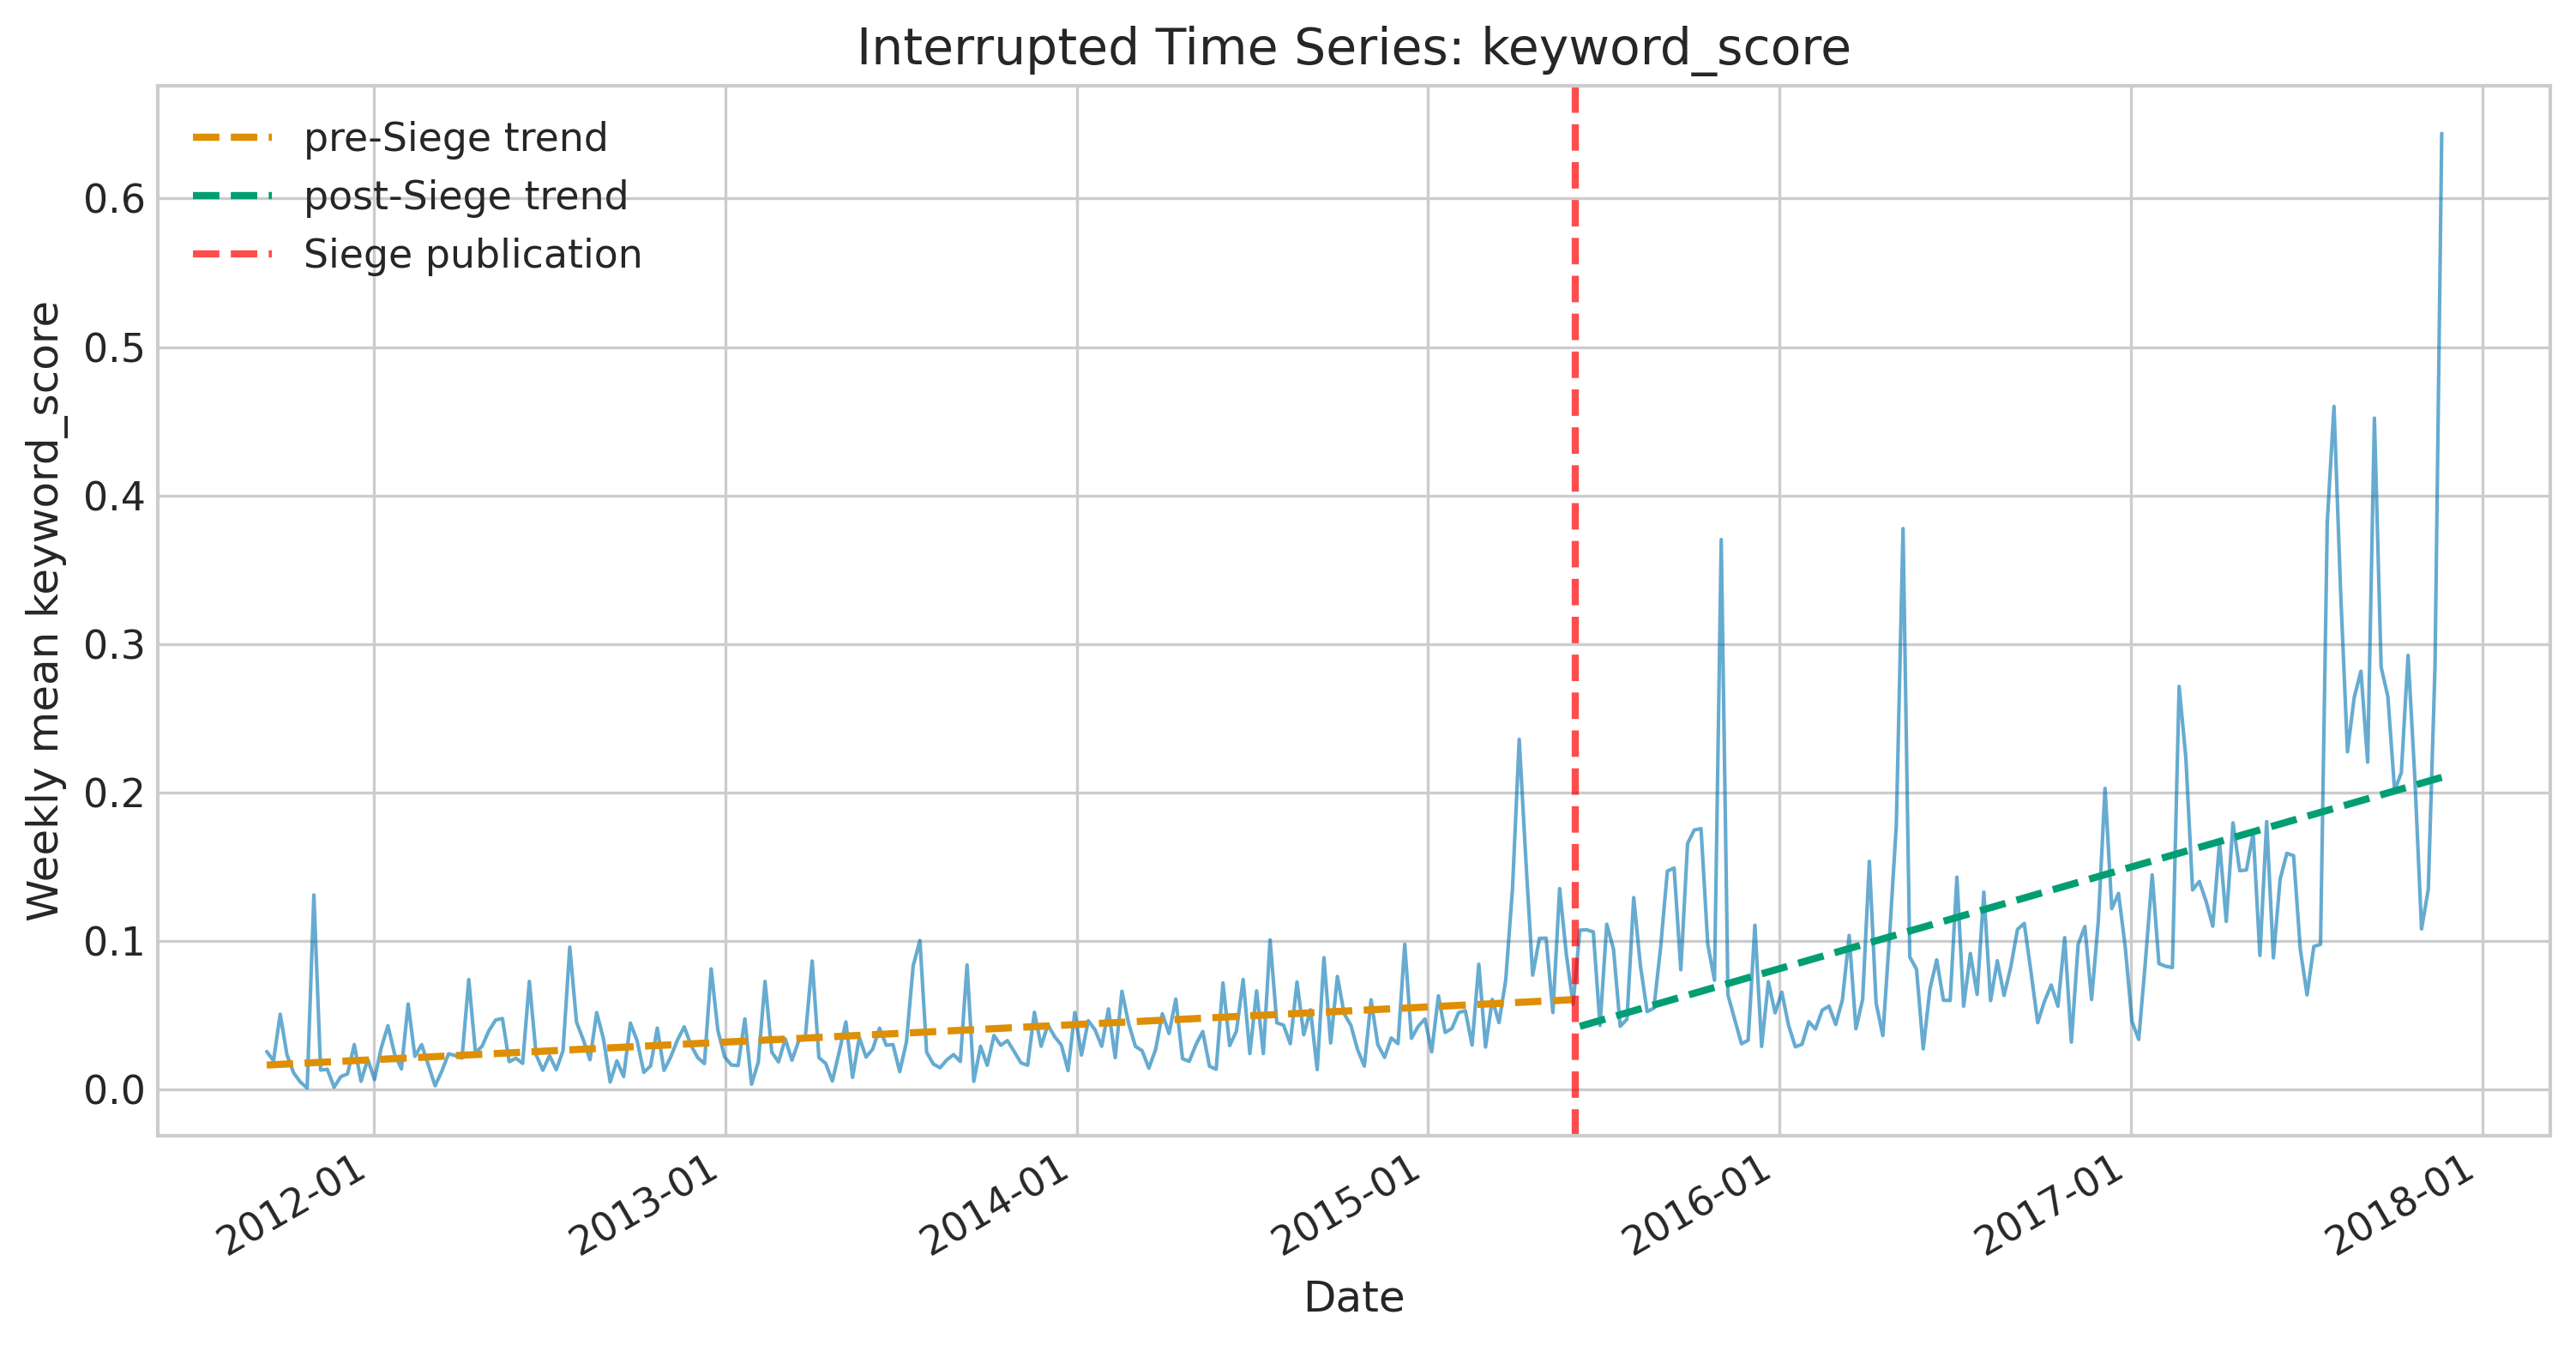
\includegraphics[width=0.85\linewidth]{its_forum_keyword_score.png}
    \caption{Interrupted time series on weekly mean Siege keyword score in Iron March forum posts, excluding Zeiger. Vertical dashed line marks $T_0$ (Zeiger's June 3, 2015 publication). Slope change $\beta_3 = 0.00015$, $p = 0.001$, $R^2 = 0.46$.}
    \label{fig:its}
\end{figure}

The gradual, slope-driven character of this break is substantively important. A level-only break would be consistent with a brief spike of attention to a newly released book. A slope-driven break is instead consistent with ongoing, compounding interpretive work of the kind I have called collective memory-work. The change points in the PELT analysis include two before $T_0$ (June 2014, March 2015), which indicates that the pre-$T_0$ trajectory is not perfectly flat; readers should interpret $T_0$ as a decisive acceleration of an already drifting series rather than as a cold-start ignition.

\subsection{Contagion, not entrepreneurship (H2, H3, H6)}

If Zeiger's publication were driving the community directly, his weekly Siege score would Granger-cause the community's. It does not. Across lags 1 through 8, no Granger test rejects the null at conventional thresholds; the best $p$-value is $0.17$ at lag 1, and the community-to-Zeiger direction also fails to reject ($p \geq 0.88$ at all lags). Zeiger's and the community's series co-move, but there is no detectable directional flow from the entrepreneur to the crowd. The result is \textit{consistent with} decentralized adoption rather than diagnostic of it; with only 324 weekly observations and a single leader, aggregate Granger tests are underpowered against punctuated or non-linear influence channels such as thread creation, pinning, and moderation. Figure \ref{fig:zeiger_comm} plots Zeiger's weekly Siege activity against the rest of the community's mean score over the Iron March period.

\begin{figure}
    \centering
    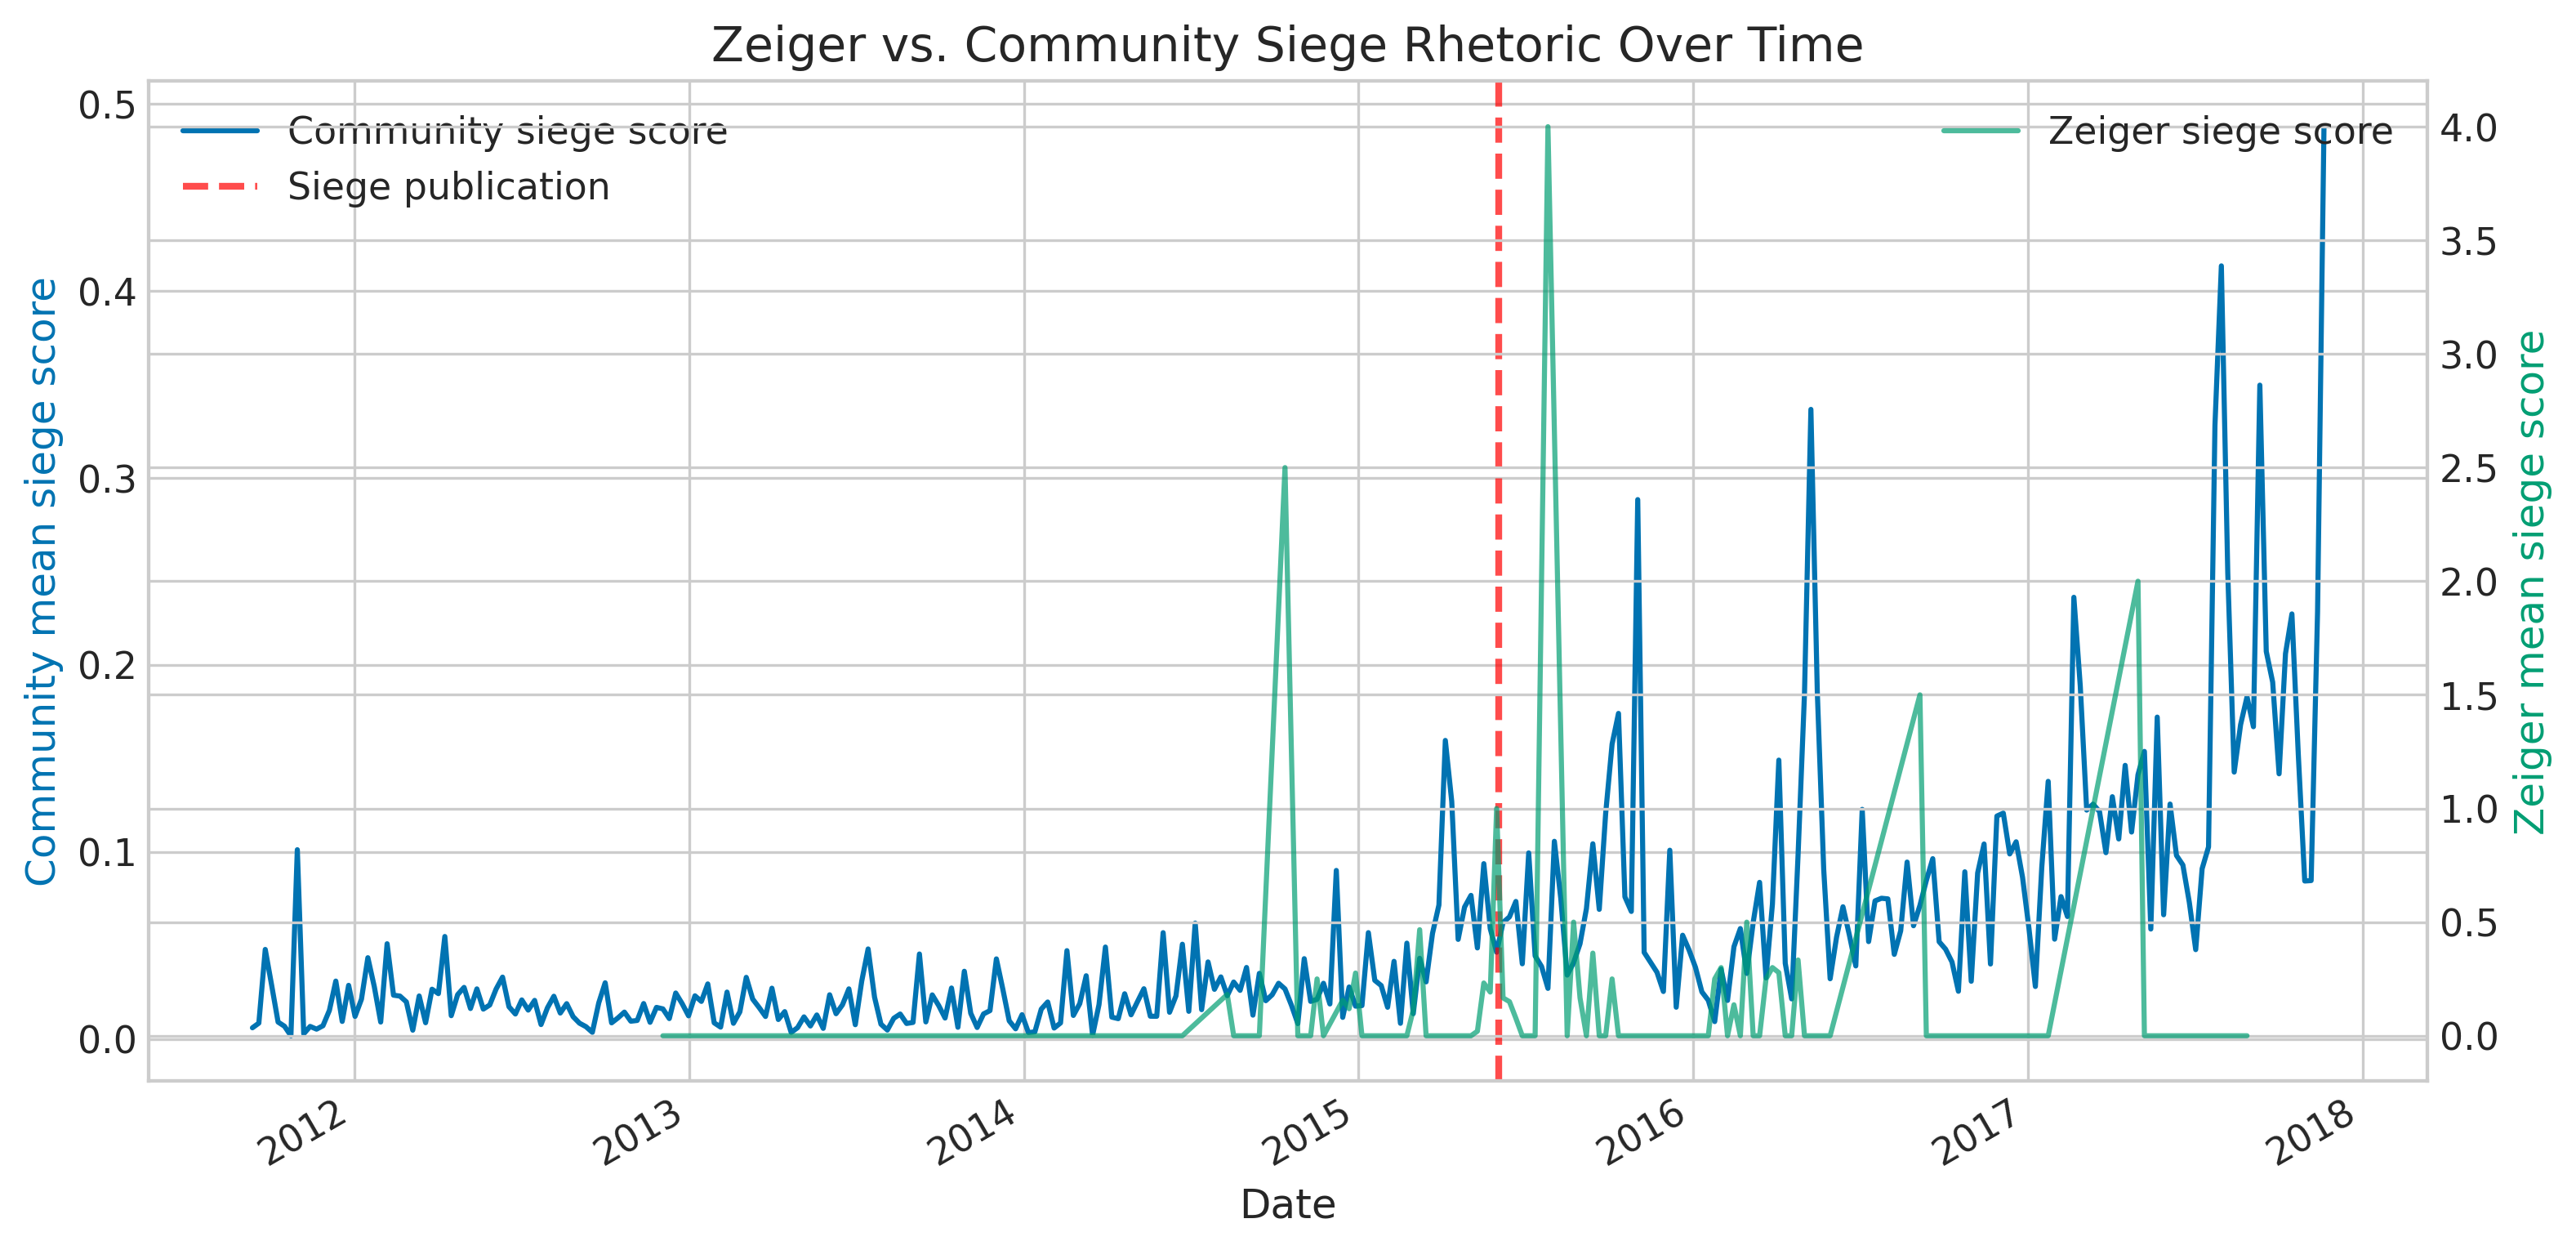
\includegraphics[width=0.85\linewidth]{zeiger_vs_community.png}
    \caption{Weekly Siege keyword score: Zeiger versus the rest of the Iron March community. The two series co-move but Granger tests do not reject the null in either direction.}
    \label{fig:zeiger_comm}
\end{figure}

What does predict adoption is network exposure. Table \ref{tab:contagion} reports a two-way fixed-effects panel regression of user-month Siege scores on lagged mean Siege score among neighbors in each of three networks. Forum co-participation exposure is strongly predictive ($\beta = 1.13$, $p < 0.001$; node-label permutation $p = 0.00$), while direct-message and reputation exposures are not. The pattern is consistent with Siege rhetoric spreading primarily in public semi-anonymous thread discussions rather than through private channels or reputation-based micro-endorsements.

\begin{table}[t]
    \centering
    \caption{Panel regression of user-month Siege score on lagged network exposure. Two-way (user $+$ month) fixed effects via within-transformation. Permutation $p$-values use 200 node-label permutations of the observed network. $N=8{,}870$ user-months across 641 users.}
    \label{tab:contagion}
    \small
    \begin{tabular}{lrrr}
    \toprule
    Predictor & Coef & $p$ & Perm $p$ \\
    \midrule
    Forum co-participation exposure & $1.131$ & $<0.001$ & $0.00$ \\
    DM exposure & $-0.040$ & $0.394$ & $0.44$ \\
    Reputation exposure & $-0.057$ & $0.695$ & $0.51$ \\
    \midrule
    $R^2$ & $0.039$ & & \\
    \bottomrule
    \end{tabular}
\end{table}

The Cox proportional-hazards results in Table \ref{tab:cox} reinforce this picture. Users with higher degree centrality in the forum co-participation network adopt Siege rhetoric substantially faster (hazard ratio $= 2.92$, $p < 0.001$), while betweenness centrality is associated with \textit{slower} adoption ($HR = 0.64$, $p < 0.001$). The split between degree and betweenness is theoretically revealing. High-degree users sit inside dense clusters of discussion and are directly exposed to canonical speech; high-betweenness users sit at structural bridges between clusters and are disproportionately bridge-keepers rather than true believers. Reputation score is not a significant predictor after adjusting for structural position. Figure \ref{fig:survival} visualizes the resulting difference in adoption trajectories between above- and below-median degree users.

\begin{table}[t]
    \centering
    \caption{Cox proportional-hazards model of time to first high-Siege post. Standardized covariates; partial-likelihood standard errors.}
    \label{tab:cox}
    \small
    \begin{tabular}{lrrrr}
    \toprule
    Covariate & Coef & HR & SE & $p$ \\
    \midrule
    Degree centrality & $1.073$ & $2.925$ & $0.066$ & $<0.001$ \\
    Betweenness centrality & $-0.446$ & $0.640$ & $0.091$ & $<0.001$ \\
    Reputation & $-0.026$ & $0.975$ & $0.056$ & $0.644$ \\
    \bottomrule
    \end{tabular}
\end{table}

\begin{figure}
    \centering
    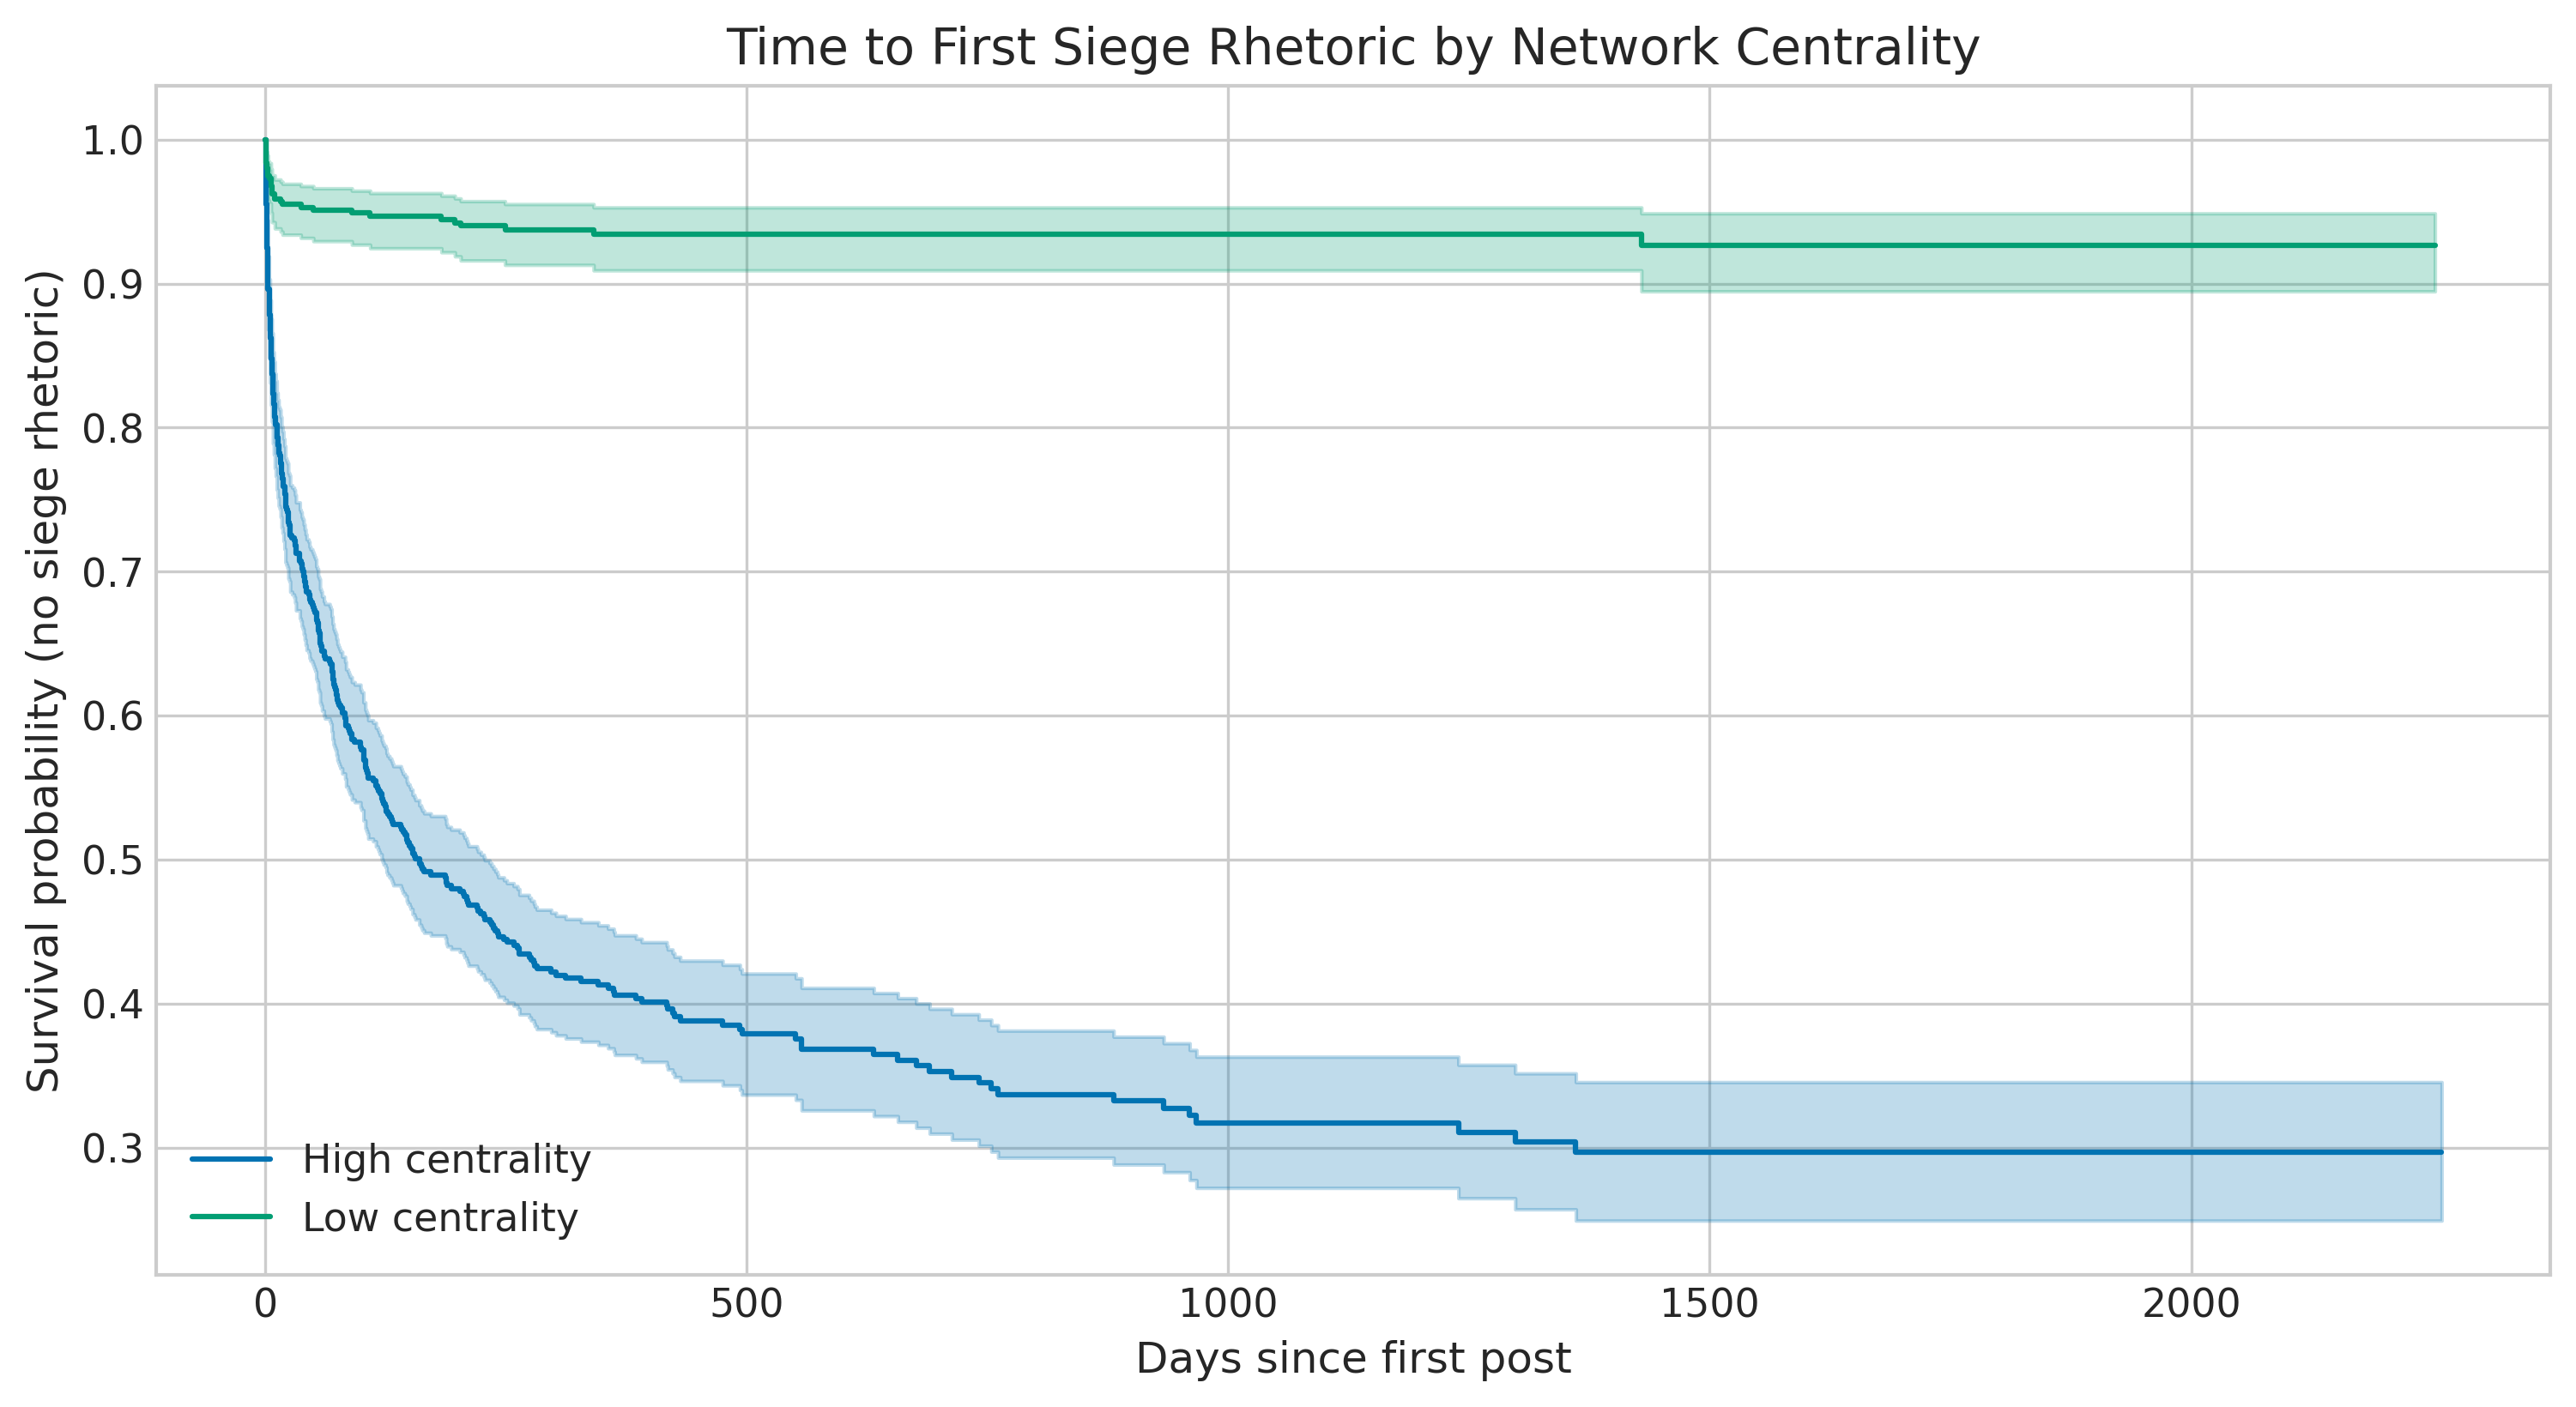
\includegraphics[width=0.85\linewidth]{survival_centrality.png}
    \caption{Cox proportional-hazards survival curves for time to first high-Siege post, stratified by degree centrality (above versus below the sample median) in the forum co-participation network.}
    \label{fig:survival}
\end{figure}

\subsection{Cohort and pipeline effects (H4, H5)}

If Siege rhetoric is a network-transmitted ideology rather than a label users arrive with, users who joined Iron March before $T_0$ should experience detectable conversion after $T_0$, and new users who joined after $T_0$ should arrive already saturated with Siege rhetoric. Both predictions hold. Among 152 pre-$T_0$ joiners with posts both before and after $T_0$, the mean user-level change in Siege score is $+0.041$ ($t = 2.26$, $p = 0.025$; Wilcoxon $p = 0.017$). Entry-level comparison is even sharper: among post-$T_0$ joiners, the mean Siege score on their \textit{first} posts is $0.184$, compared to $0.022$ for pre-$T_0$ joiners' first posts (Mann-Whitney $p < 0.001$). Post-2015 Iron March was, in effect, recruiting a different kind of user.

A subtler prediction concerns the forum-to-DM pipeline. If Siege rhetoric originates in private conversation and then leaks into public space, users would talk about it in DMs first. The opposite is true: among 190 users who used Siege-related language in both DMs and forum posts, 83.7 percent did so in the forum first, while only 10.0 percent did so in DMs first ($t$-test $p < 0.001$). The mean DM-minus-forum lead is $-177$ days. Siege-talk was a public performance, which is itself theoretically informative. Canonization is an inherently public act of status-elevation, and collective memory-work requires an audience. The forum-first pattern is exactly what the theory would predict if Siege rhetoric were functioning as a public marker of canon alignment rather than as a private confidence.

\subsection{Canonization, exegesis, and spatial concentration (H7, H10, H11)}

The canonization mechanism is sharply supported. Of 194,652 analyzed forum posts, 7,358 score above the Siege threshold. Siege posts receive a mean of 2.335 reputation points versus 1.342 for non-Siege posts (Mann-Whitney $p < 0.001$). Estimating a negative binomial regression of reputation counts on a Siege indicator, controlling for log post length and with month fixed effects, yields a coefficient of $0.429$ ($p < 0.001$), corresponding to an incidence rate ratio of $1.54$. Siege-aligned posts receive, on average, 54 percent more reputation points than otherwise similar non-Siege posts of comparable length. The community does not merely tolerate Siege rhetoric; it rewards it. Figure \ref{fig:reputation} shows the distribution of reputation for Siege versus non-Siege posts and the monthly mean-reputation trajectory over the forum's lifespan.

\begin{figure}
    \centering
    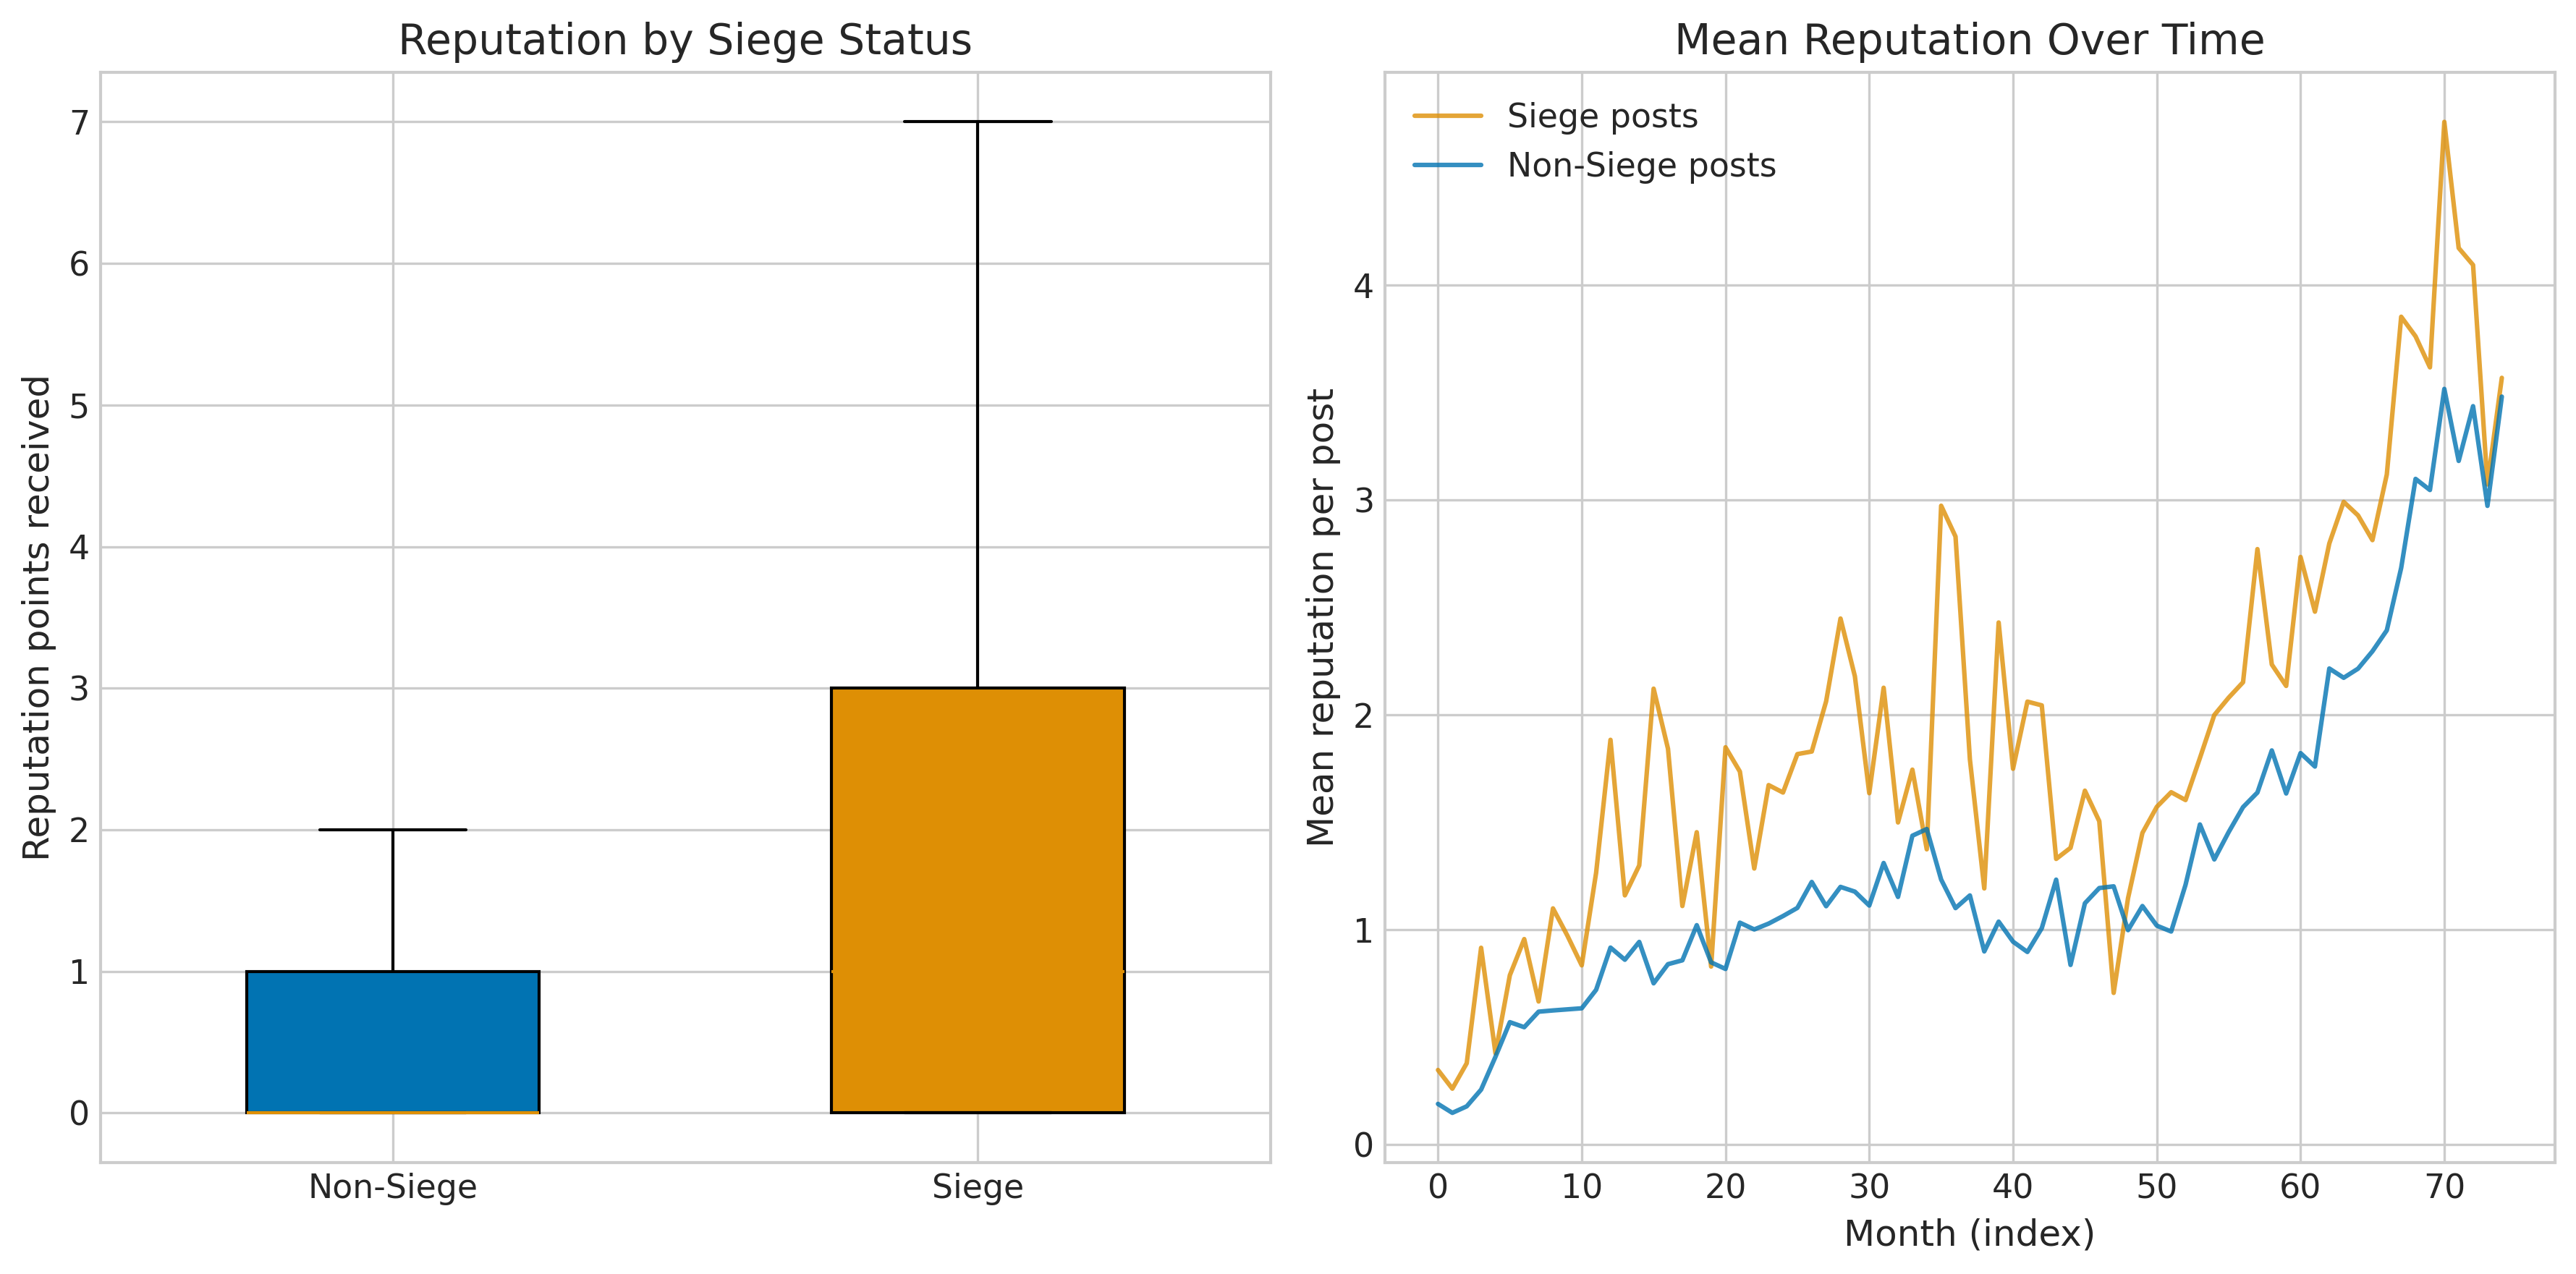
\includegraphics[width=0.85\linewidth]{reputation_reinforcement.png}
    \caption{Reputation received by Siege versus non-Siege posts on Iron March. Left: distribution of reputation points by Siege status. Right: monthly mean reputation per post by Siege status over time, showing a persistent gap. Negative binomial regression with month fixed effects and log post length yields $IRR=1.54$, $p<0.001$.}
    \label{fig:reputation}
\end{figure}

The spatial concentration mechanism is also supported. The Herfindahl-Hirschman Index of Siege rhetoric across 87 subforums rises from $0.050$ pre-$T_0$ to $0.116$ post-$T_0$. The top five subforums by pre-to-post increase in Siege prevalence are \texttt{archive-project-central} ($+0.176$), \texttt{articles} ($+0.156$), \texttt{antimony-group} ($+0.139$), \texttt{deutschland-austria} ($+0.131$), and \texttt{books} ($+0.114$). Among this top group, the interpretive and archival subforums (\texttt{archive-project-central}, \texttt{articles}, \texttt{books}, plus \texttt{external-materials-archive} and \texttt{adminship-center} just outside the top five) predominate; the regional and project-specific subforums (\texttt{deutschland-austria}, \texttt{antimony-group}) indicate that Siege content also seeded national and operational discussion spaces. The single highest post-$T_0$ Siege-prevalence subforum, \texttt{hall-of-graduates}, contains posts celebrating users who have ``graduated'' into offline militant activity. The shape of Siege discourse concentrates in the spaces where interpretation, curation, and initiation happen. Figure \ref{fig:subforums} summarizes the pre-to-post prevalence shift across subforums.

\begin{figure}
    \centering
    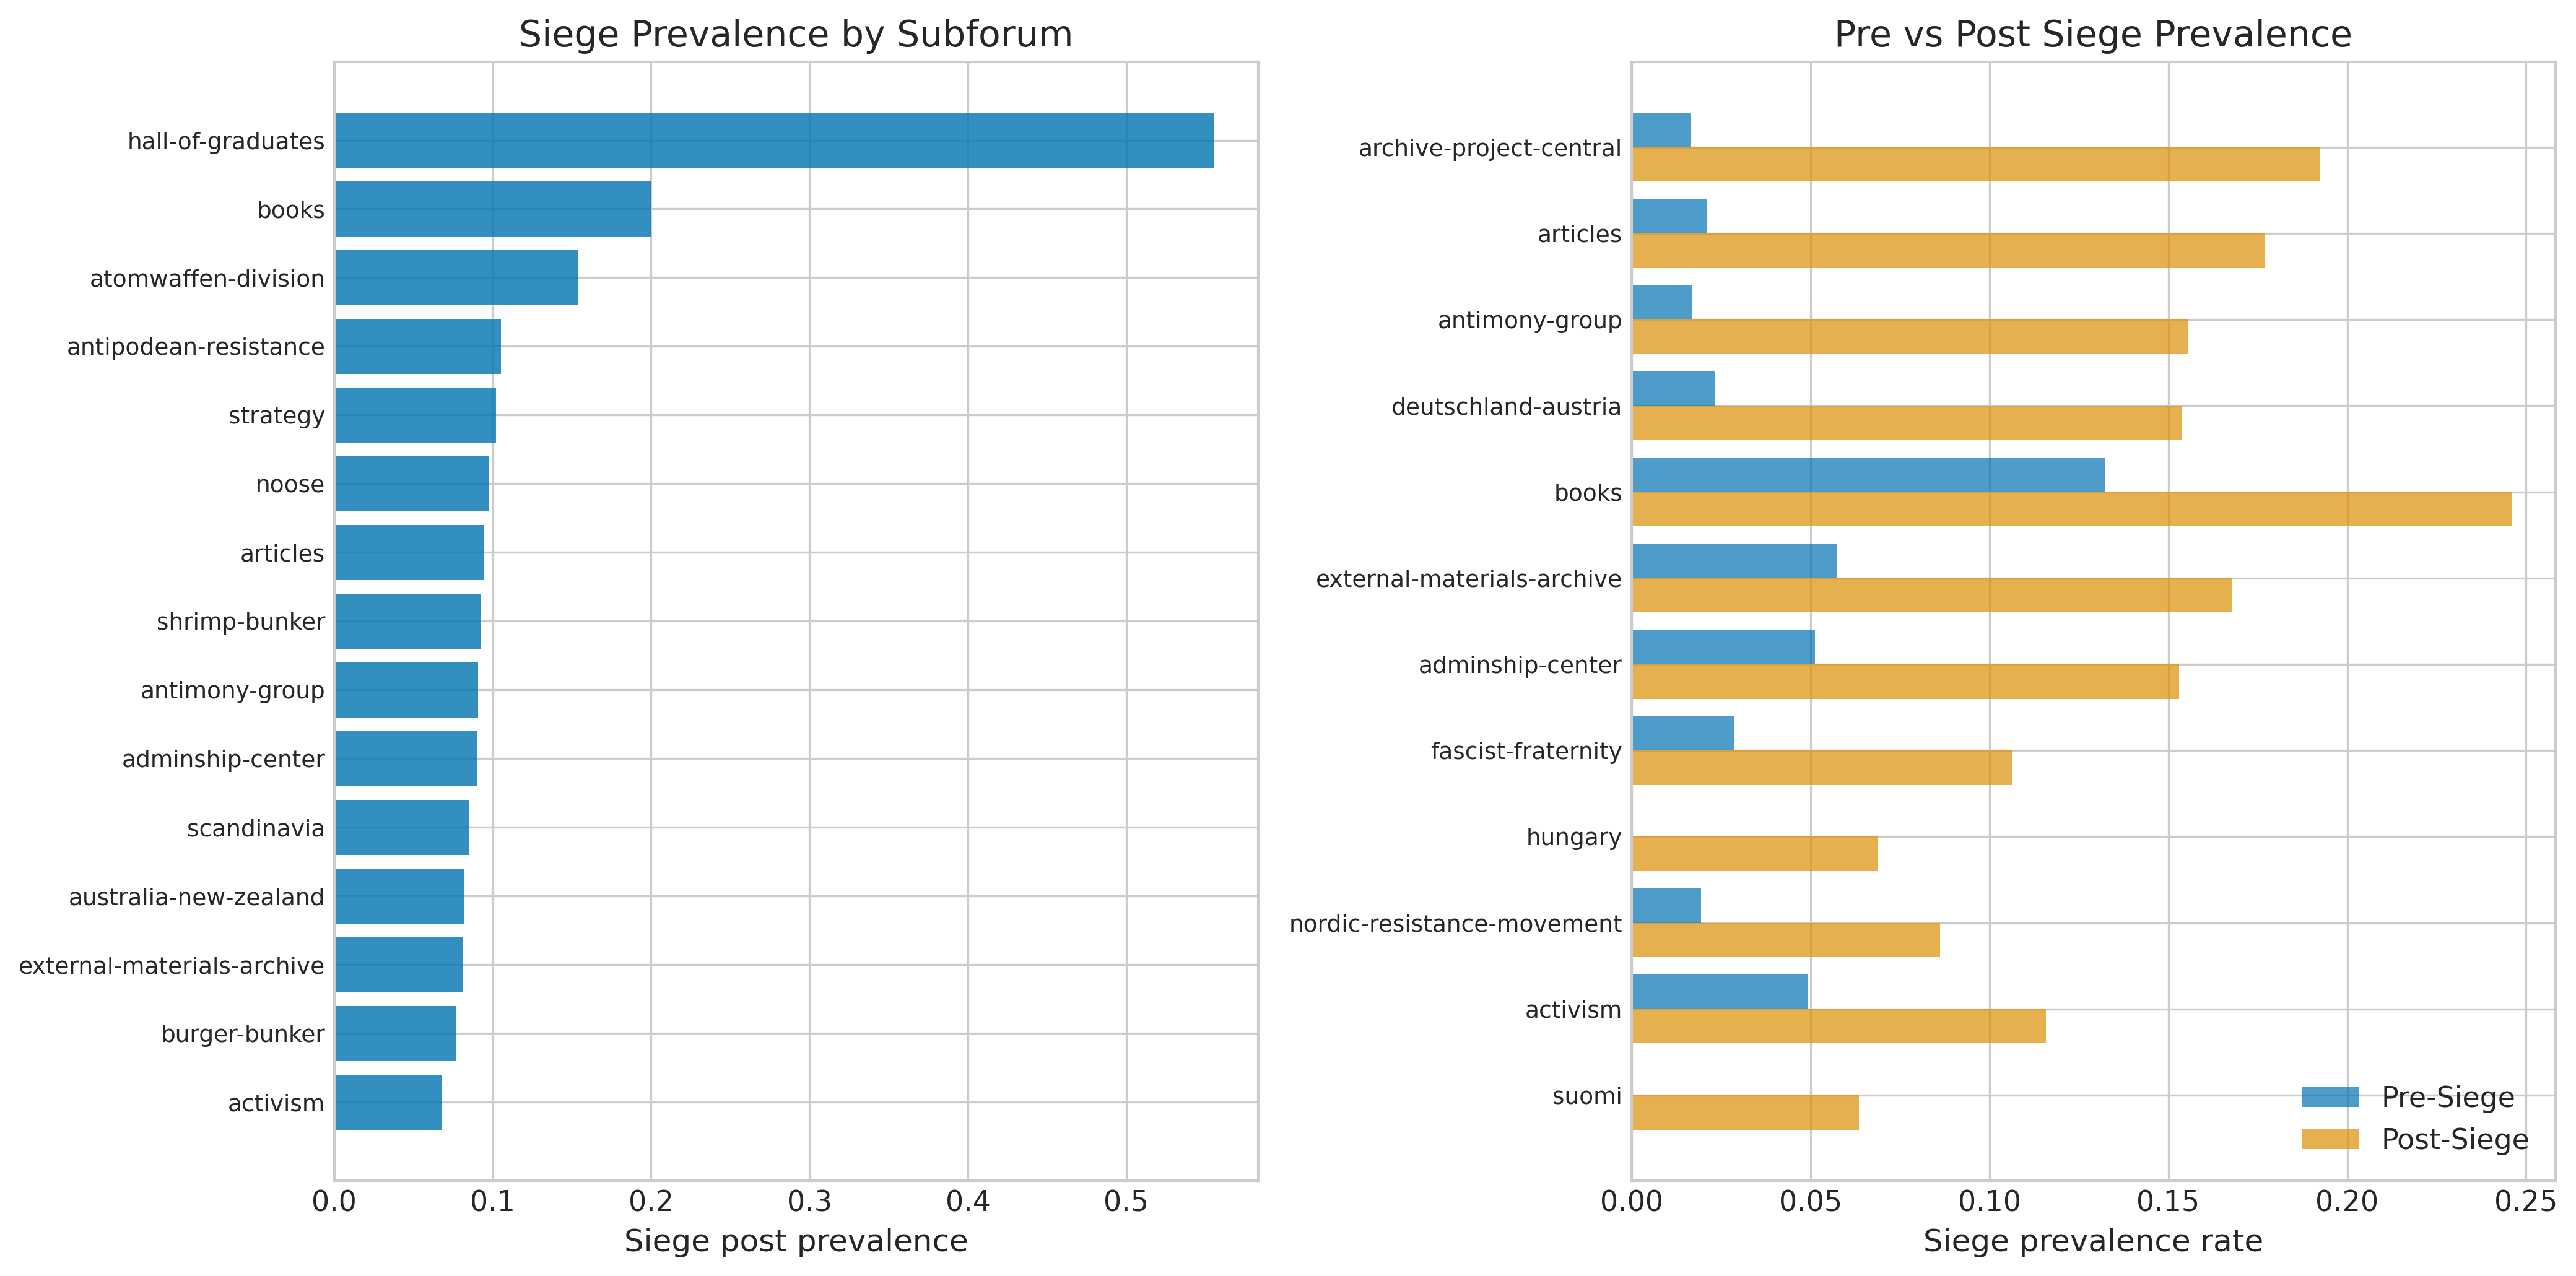
\includegraphics[width=0.85\linewidth]{subforum_diffusion.png}
    \caption{Pre- and post-treatment Siege prevalence across the top subforums by pre-to-post change. Concentration shifts toward interpretive and archival spaces.}
    \label{fig:subforums}
\end{figure}

Semantic convergence offers a more ambivalent picture. The monthly coefficient of variation of user-level Siege scores shows both a significant positive level change at $T_0$ ($\beta_2 = 3.41$, $p = 0.009$) and a significant negative slope change ($\beta_3 = -0.054$, $p = 0.011$). The level change indicates that immediately after $T_0$, users become more heterogeneous in how much Siege rhetoric they use: some enthusiasts sharply intensify while others do not move. The negative slope change indicates that this heterogeneity then declines over the following months. Post-$T_0$ heterogeneity falls back toward, but does not fall below, the pre-$T_0$ mean within the forum's remaining lifespan: the pre-versus-post mean CV comparison is $1.45$ vs $1.73$ and is not statistically significant ($p = 0.12$). The convergence result should therefore be read as tentative evidence of a late-onset compression rather than a clean dichotomous shift, and future work on successor platforms should test whether the compression continues beyond the Iron March observation window. Figure \ref{fig:semantic} visualizes the CV trajectory.

\begin{figure}
    \centering
    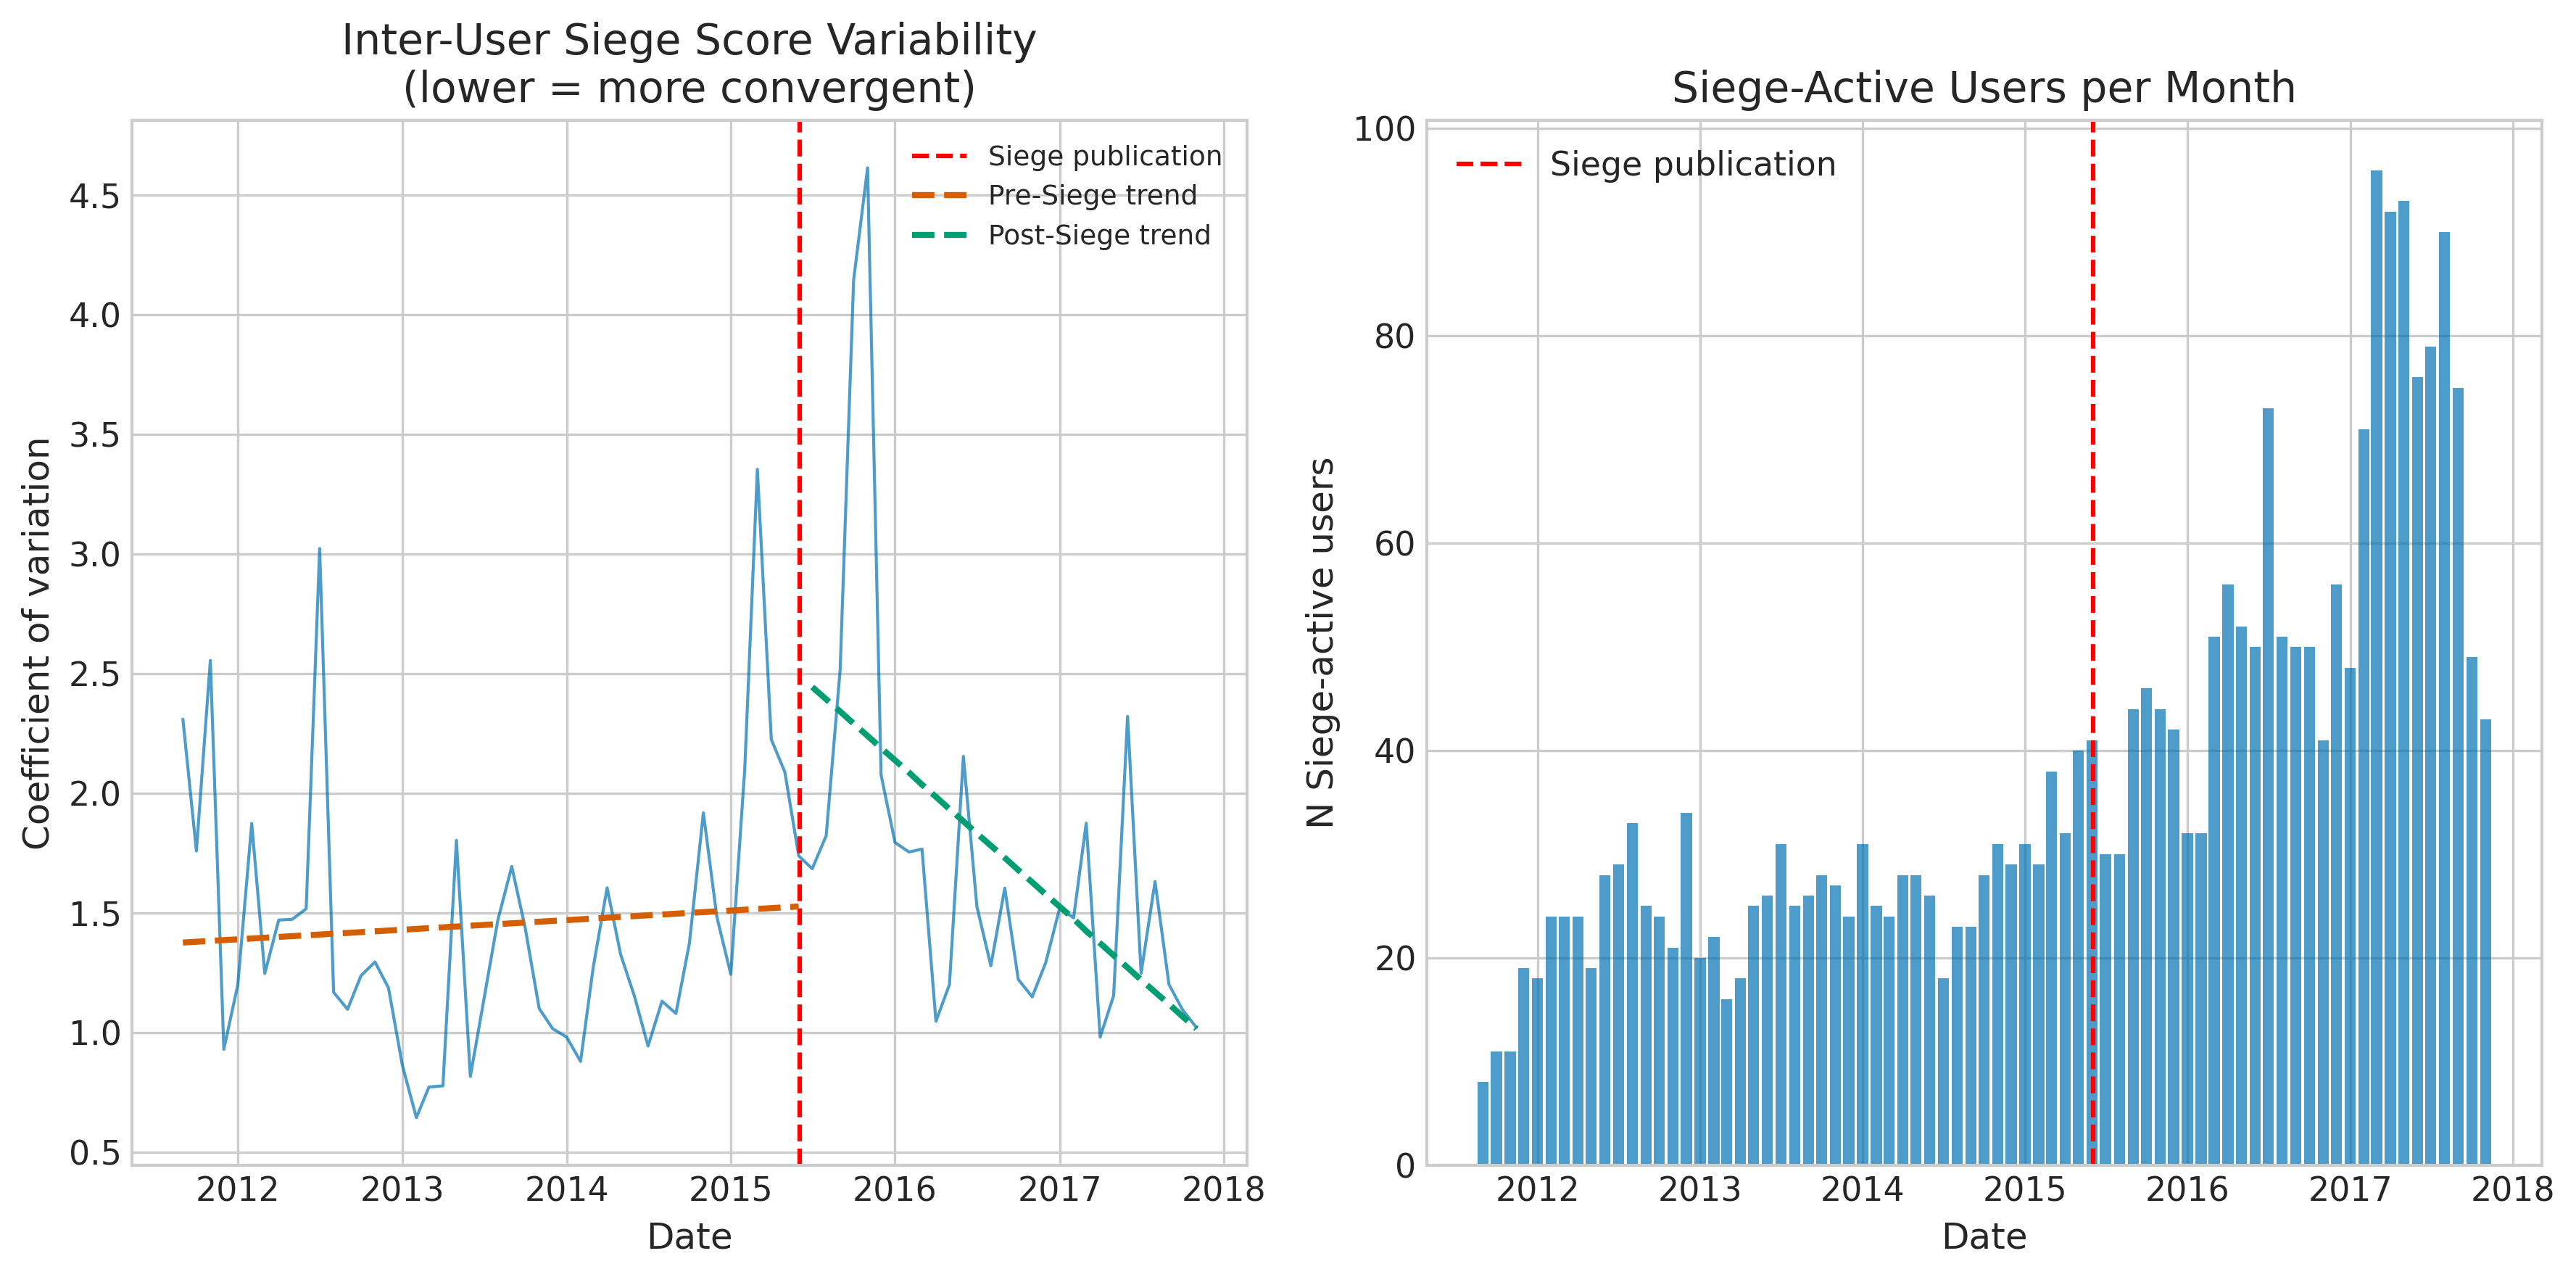
\includegraphics[width=0.85\linewidth]{semantic_convergence.png}
    \caption{Monthly coefficient of variation of user-level Siege scores (left) and count of Siege-active users per month (right). Post-$T_0$, the CV rises and then declines, consistent with an initial burst of heterogeneous enthusiasm followed by gradual compression; the right panel documents the rising size of the active population.}
    \label{fig:semantic}
\end{figure}

\subsection{Summary scorecard}

Table \ref{tab:scorecard} summarizes the 11 primary hypothesis tests reported above. Internal contagion, canonization, and spatial concentration are supported; top-down entrepreneurship is not. Applying Benjamini-Hochberg FDR correction at $q=0.05$ across the 11 correlated tests leaves all findings with naive $p < 0.01$ intact (their BH-adjusted $q$-values remain below $0.05$), while the borderline cases (H4 at $p=0.025$, H9 at $p=0.087$, and the H10 level change at $p=0.009$) should be read as marginal; H9 in particular does not survive even conservative correction. I report adjusted $q$-values alongside raw $p$-values in the replication materials.

\begin{table}[t]
    \centering
    \caption{Hypothesis scorecard. ``$\checkmark$''~$=$ supported, ``$\sim$''~$=$ partial or marginal, ``$\times$''~$=$ not supported.}
    \label{tab:scorecard}
    \tiny
    \begin{tabular}{clll}
    \toprule
    \# & Hypothesis & Verdict & Key statistic \\
    \midrule
    H1 & \textit{Siege} publication $=$ structural break & $\checkmark$ & $\beta_3=0.00015$, $p=0.001$ \\
    H2 & Network exposure predicts adoption & $\checkmark$ & $\beta=1.13$, $p<0.001$ \\
    H3 & Zeiger Granger-causes community & $\times$ & best $p=0.17$ \\
    H4 & Cohort conversion effects & $\checkmark$ & $t=2.26$, $p=0.025$ \\
    H5 & Forum-first pipeline & $\checkmark$ & 83.7\% forum-first \\
    H6 & Degree centrality accelerates adoption & $\checkmark$ & $HR=2.92$, $p<0.001$ \\
    H7 & Community rewards Siege speech & $\checkmark$ & $IRR=1.54$, $p<0.001$ \\
    H8 & Within-thread escalation (linear) & $\sim$ & catalyst pattern, not linear \\
    H9 & Thread exposure $\to$ adoption & $\sim$ & $\beta=0.144$, $p=0.087$ \\
    H10 & Semantic convergence (slope) & $\checkmark$ & $\beta_3=-0.054$, $p=0.011$ \\
    H11 & Subforum concentration & $\checkmark$ & HHI $0.050 \to 0.116$ \\
    \bottomrule
    \end{tabular}
\end{table}

\section{Discussion}

\subsection{Collective Memory-Work, Not Ideological Entrepreneurship}

A defining finding of this paper is that the single most visible individual in the Iron March Siege story, Zeiger himself, does not Granger-cause the community's rhetoric. The result is consistent with decentralized adoption rather than direct entrepreneurship, though it is not by itself conclusive. Weekly aggregate Granger tests are underpowered against punctuated or non-linear channels of influence such as thread creation, pinning, and moderation, and a more powerful test of direct influence would exploit thread-level rather than weekly data. What the aggregate null does rule out is a simple broadcasting model in which Zeiger's weekly posting activity reliably leads the community's.

What does predict community adoption is network exposure within the forum co-participation graph. Degree-central users adopt fastest; new members arrive already saturated with Siege language; Siege-aligned posts receive 54 percent more reputation than otherwise comparable posts. Reputation reinforcement is the observable signature of canonization; spatial concentration in interpretive subforums, together with late-onset semantic convergence, marks exegesis; network-exposure-driven adoption marks contagion. The three signatures appear jointly in the 2015--2017 trajectory.

Substantively, this reframes Iron March's political significance. Iron March mattered not because Slavros or Zeiger or any other individual was a particularly charismatic ideologue, but because the forum's institutional design made it possible for a decentralized community to collectively elevate, interpret, and reinforce a memory artifact. The resulting identity proved durable enough to survive the 2017 shutdown.

\subsection{Returning to the Puzzle}

The collective-action puzzle posed in Section 2 asked how communities lacking hierarchy, formal membership, or persistent command structure nonetheless produce coordinated offline action. Classical resource-mobilization theory \citep{mccarthy1977resource, tilly2017mobilization, olson1971logic} identifies organization as the solution. The memory-artifact account developed here suggests a functional substitute. The artifact performs some of the coordinating work that a formal organization would otherwise do: it supplies a shared narrative, a common vocabulary, a status hierarchy keyed to canon alignment, and an interpretive agenda that can be worked on collectively without central direction. In this sense the memory artifact is not a replacement for the substrate of institutional rules, but a lightweight mechanism that lets a modest substrate do outsized coordination work. This complements rather than displaces the collective-learning account \citep{kenney2020community, lee2022, furstenberg2024decentralized}, which explains how tactical expertise circulates; what the memory-artifact view adds is an explanation for how a durable, action-oriented identity stabilizes in the absence of organizational enforcement.

\subsection{Implications for the study of online extremism}

The findings have three implications for existing scholarship. First, influence-centric models of radicalization that locate ideological change in the activity of specific ``entrepreneurs'' or ``propagandists'' are under-specified for this class of community. Zeiger is the most visible single individual in the Iron March Siege story, yet at the weekly resolution his posting does not lead the community's; what does is exposure within a dense public forum graph. Second, the Ostromian institutional-design literature \citep{ostrom1990governing, frey2019_part, schneider2022} and the communities-of-practice literature \citep{kenney2020community, furstenberg2024decentralized, lee2022} offer complementary rather than rival accounts: the Charter provides the procedural substrate and communities of practice circulate tactical expertise, while memory-work is what stabilizes a durable action-oriented identity on top of that substrate. Iron March is distinctive relative to forums such as Stormfront not in having an institutional substrate \citep{caren2012social, bowman2009}, which Stormfront also has, but in coupling that substrate with an ideologically programmatic Charter and a concentrated exegetical apparatus around a single canonized text. Third, the framework offers a bridge between qualitative and quantitative work on online radicalization: qualitative accounts of Iron March and its successors have consistently emphasized the centrality of specific texts and memory practices \citep{upchurch, johnson2023siege, sunshine2024neo, ware2019siege}, and the statistical pipeline developed here shows that those qualitative observations have measurable structural analogues in the forum corpus itself.

\subsection{Limitations}

Several limitations qualify the conclusions. First, network contagion models are known to be susceptible to homophily confounds \citep{aral2009distinguishing, shalizi2011homophily}: users who are already ideologically similar cluster together, which can generate apparent contagion even in the absence of influence. I address this partially through user fixed effects and node-label permutation tests. Both are consistent with a true influence effect, but neither fully resolves latent-attribute homophily, and causal identification in observational network data remains inherently limited. The node-label permutation test addresses structural coincidence rather than latent-attribute selection; a stronger design would add lagged-own-score controls to the panel and, where feasible, instrumented-exposure estimators of the Bramoull\'e-Djebbari-Fortin type. A related issue, flagged in Section 3.1, is that the contagion test (H2, H6) and the spatial-concentration test (H11) are both observed on the forum co-participation graph and are partially entangled: a user who is pulled into an interpretive subforum is simultaneously exposed to Siege-aligned alters and to the venue of exegesis, so the two effects are not cleanly separable. A design with thread-level fixed effects in the contagion panel would attenuate the entanglement and is flagged as a revision target.

Second, the Siege rhetoric measure inherits the biases of its underlying lexicon and embedding model. The specific weights and thresholds were chosen based on corpus-level hit rates and qualitative review rather than an external gold-standard annotation, and while the measure is face-valid and robust to the ``siege'' overloading problem by the embedding boost, it has not been validated against a hand-coded benchmark with reported precision, recall, or inter-annotator agreement. A measurement appendix with human coding of a stratified subsample, alternative embedding encoders (e.g., \texttt{all-mpnet-base-v2}, a TF--IDF baseline), and lexicon ablations (Tier 1 only; randomized Tier 3 weights) is a first-priority revision target.

Third, the interrupted time-series design is vulnerable to misspecification of the pre-trend, which the pre-$T_0$ PELT breaks in 2014 and 2015 exacerbate. The post-$T_0$ effect should therefore be read as an acceleration of an already-drifting series rather than as a cold-start ignition. A reviewer-grade revision would add placebo ITS estimates on 500 randomly drawn pre-treatment dates, bandwidth sensitivity (dropping the first/last 6, 12, and 26 weeks), a piecewise-linear or quadratic pre-trend specification, and a difference-in-differences comparison against a contemporaneous non-accelerationist forum. I flag these as revision targets.

Fourth, the Cox proportional-hazards model reports hazard ratios without diagnostic tests of the proportional-hazards assumption or time-varying specifications of centrality, both of which are plausibly violated in a forum where post-adoption activity inflates degree. The betweenness coefficient sign (HR $=$ 0.64, slower adoption) was not prespecified and should be treated as exploratory.

Fifth, the Ukraine-war pipeline is a plausible parallel driver of the 2014--2015 pre-$T_0$ drift that this design cannot fully separate from the internal memory-work dynamics. Iron March members were heavily represented in the Misanthropic Division / Azov recruitment network during the same period, and their combat tourism plausibly co-produced the escalation in Siege-adjacent rhetoric that PELT detects before $T_0$ \citep{colborne2022fires}. I cannot rule out that the 2015 Zeiger publication was itself an artifact of this pipeline rather than an independent canonization shock.

Sixth, the direct-message corpus (approximately 21,700 messages) is much smaller than the forum corpus (approximately 195,000 posts), which means DM-based analyses may lack statistical power. The forum-first pipeline result should be interpreted in that light, though the effect size (83.7 percent forum-first) is large enough that the power limitation is unlikely to be determinative.

Seventh, the reputation data has not been independently validated against Iron March's original database schema beyond the joins described in the methods section. The H7 reputation reinforcement result holds across specifications but should be interpreted cautiously.

Eighth, the paper restricts its empirical scope to Iron March-internal dynamics. Whether the memory artifact produced in Iron March persists, travels, or amplifies on downstream platforms after the November 2017 shutdown is a natural extension, discussed in the Conclusion as a direction for future work rather than tested here.

\section{Conclusion}

Despite decentralization, fluid membership, and a resistance to operating as a movement itself, Iron March was a connection (and sometimes origin) point for some of the most influential neo-fascist militant groups of the past two decades. It hosted activists from Ukraine's Azov Movement, Greece's Golden Dawn, Italy's CasaPound, the United Kingdom's National Action, and Scandinavia's Nordic Resistance Movement. Its members kickstarted a family tree of new groups, including the Siege Culture terrorist formations Atomwaffen Division, Feuerkrieg Division, Sonnenkrieg Division, and The Base, alongside adjacent (though not direct-lineage) alt-right street formations such as Vanguard America and the Rise Above Movement \citep{newhouse2021threat, ware2019siege, sunshine2024neo}. The ability for loose, non-hierarchical, decentralized ``digital campfires'' like Iron March to nonetheless provide support for overcoming collective-action problems remains a puzzle for the study of political violence: why does coordinated, motivated, and violent offline action emerge from some online spaces and not others?

This paper has argued that collective memory formation provides a tractable mechanism for answering that question, and that the 2015 republication of James Mason's \textit{Siege} on Iron March is a useful case for demonstrating the argument. Using a multi-stage analysis pipeline on the leaked Iron March database, the results show that the publication produced a persistent structural break in forum rhetoric (H1), that the rhetoric diffused through network exposure rather than through Zeiger's direct influence (H2, H3, H6), that cohorts joining after the publication arrived already saturated with Siege language and pre-existing members converted in measurable numbers (H4, H5), that the community rewarded Siege-aligned speech with more reputation (H7), that rhetoric concentrated in interpretive subforums (H11), and that inter-user language briefly diverged and then compressed (H10). Across a battery of 11 primary tests, the pattern is consistent with collective memory-work as the central mechanism.

The central implication deserves emphasis. Online extremist mobilization is not reducible to top-down messaging. The single most visible entrepreneur in the Iron March Siege story does not Granger-cause the community's rhetoric at weekly resolution; what predicts individual adoption is exposure within a dense public forum graph, reputation-reinforced canonization, and spatially concentrated exegesis. Models of radicalization that focus exclusively on influencers miss this.

\subsection*{Future Directions}

Two extensions follow directly from the framework and are natural next steps.

First, the \textit{portability corollary} developed in Section 3 but not tested here predicts that because collective memory lives in a portable textual artifact rather than in the platform that produced it, destroying the platform should redistribute the memory across receiving platforms rather than eliminate it. The November 2017 Iron March shutdown is the event that enables this test. Candidate receiving platforms include 4chan's /pol/ board, Telegram-based Terrorgram channels, Gab, and successor forums such as Fascist Forge. A fuller cross-platform design would combine vocabulary-level temporal priority tests, URL-domain diffusion, per-sub-theme Granger analyses, and an ITS on the shutdown date itself. Null results on some platforms alongside positive results on others would be informative about \textit{where} the diaspora migrated, not only whether the artifact survived. Data-access constraints make this non-trivial; the /pol/ archive is one of the few long-running far-right platforms for which a full Asagi-schema dump is publicly available \citep{hine2017kek, papasavva2020raiders}, but Telegram and successor forum data are increasingly tractable.

Second, the three-mechanism framework makes comparative predictions that remain to be tested. Stormfront, for example, hosts canonical texts but does not appear to generate the spatial concentration of interpretive activity that Iron March did, which may help explain its comparatively weaker record of producing offline mobilization \citep{caren2012social, bowman2009}. The Terrorgram network on Telegram does exhibit concentrated exegesis around curated ``manifesto'' texts, which would predict stronger mobilization outcomes, consistent with the documented record of Terrorgram-linked attacks \citep{newhouse2021threat, colin2024and}. Fascist Forge similarly organizes around the \textit{Siege} canon but with different moderation and reputation architectures \citep{lee2022}. A comparative design across Stormfront, Iron March, Terrorgram, Fascist Forge, and Gab, applying the same measurement pipeline developed here, would allow direct tests of the framework's generalizability and its scope conditions.

Online communities have increasingly influenced far-right political violence, and more scholarly attention to the specific social processes that bind decentralized memory communities together may help explain why some forums produce coordinated offline action and others do not.

%% Use \bibliography{...} if using BibTeX
\bibliography{sample}

%TC:subst \printbibliography \bibliography
%TC:macro \field [0,1]
%TC:macro \name [0,0,0,1]
%TC:macro \list [0,0,1]
%% Use \printbibliography if using BibLaTeX
% \printbibliography

\end{document}
